\documentclass[a4paper]{article}

\usepackage[francais]{babel}
\usepackage[utf8x]{inputenc}
\usepackage[T1]{fontenc}
%\usepackage{amsmath}
\usepackage{graphicx}
\usepackage[colorinlistoftodos]{todonotes}
\usepackage{comment}
\usepackage{float}
\usepackage[colorlinks=true,linkcolor=black,citecolor=black]{hyperref}
\usepackage{colortbl}





\title{\bsc{INSA} de Rennes \\ Département Informatique \\ \bigskip \hrule \bigskip Système d'annotation et de navigation dans des images d'archives \\ \bigskip Rapport de spécification fonctionnelle \bigskip \hrule}
\author{Raphaël \bsc{Baron}, Pierre-Olivier \bsc{Bouteau}, Nicolas \bsc{Charpentier}, \\ Clément \bsc{Leboullenger}, Thomas \bsc{François}, Benoit \bsc{Travers}}

\begin{document}

\maketitle
\thispagestyle{empty}

\newpage
\tableofcontents
\thispagestyle{empty}

\newpage
\section*{Introduction}

	Les Archives départementales d'Ille-et-Vilaine sont en charge de la collecte, du classement, de la conservation et de la communication des archives qui constituent une grande partie du patrimoine historique écrit du département. 
\`A l'approche du centenaire de la Première Guerre Mondiale, les Archives, en collaboration avec l'\bsc{INSA} de Rennes, ont choisi de proposer aux étudiants en quatrième année du département informatique un sujet de mise en valeur des documents li\'es \`a la Grande Guerre.

	L'objectif du projet est de construire un outil d'annotations semi-auto\-matiques des documents liés au recrutement militaire concernant cette période. L'outil doit permettre à un utilisateur, visiteur des archives, d'associer lecture et annotation du document avec l'image numérisée qui lui correspond. En plus de naviguer et d'annoter les images, l'usager peut utiliser ces annotations pour rechercher des documents, par exemple trouver une personne grâce a son nom.\\
	
	Ce rapport de spécifications fonctionnelles reprend brièvement les notions importantes abordées dans le rapport de pré-étude, avant de décrire grossièrement l'architecture générale choisie pour la réalisation de ce système. Finalement, la majeure partie de ce rapport est consacrée à la description des spécifications fonctionnelles.

\newpage

\section{Analyse du besoin}
\subsection{Projet xxx (nom appli)}
\todo{Présenter le projet ce qu'il doit faire ainsi que l'équipe}
	Dans le cadre des projets de 4éme année du département informatique, notre objectif est de développer une application permettant d’annoter des registres matricules militaires (RMM). Ces annotations doivent être à la fois simples et rapides à créer. Il sera important pouvoir visualiser des images correctement afin de pouvoir les annoter correctement. De plus, l’application devra permettre à l’utilisateur de facilement rechercher des informations liées à ces annotations. Les principales fonctionnalités à développer seront la recherche de RMM ou d’informations, la visualisation d’images et l’annotation de ces images. Sachant que notre application sera conçue pour fonctionner sur une table Microsoft PixelSense, nous utiliserons donc des émulateurs pour le développement du projet.
	Notre équipe est composée de 6 élèves ingénieurs de 4éme année du département informatique de l’INSA de Rennes : Raphaël \bsc{Baron}, Pierre-Olivier \bsc{Bouteau}, Nicolas \bsc{Charpentier}, \\ Clément \bsc{Leboullenger}, Thomas \bsc{François} et Benoit \bsc{Travers}. Nous devons prendre en compte l’absence de Thomas et Benoit lors du second semestre pour cause de mobilité internationale, l’équipe sera donc réduite à quatre étudiants pour développer le projet pendant cette période.
\subsection{Mise en valeur des documents de guerre}
\todo{Expliquer vite fait pourquoi ces docs, en mettre un de chaque en photo, dire que leur présentation est faite dans le rapport de pré-étude (notamment pour le registre)}

L'application étant destinée au centenaire de la guerre 14-18, deux types de documents nous intéressent particulièrement : le registre matricule militaire et la table des registres matricules militaires. Rappelons que ces documents étaient des documents militaires mais qui ont été donnés aux archives, ce sont les seuls documents militaires que les archives possèdent.

\subsubsection{Le registre matricule militaire}
Le RMM (Registre Matricule Militaire), dont vous trouverez un exemple complet en annexe[\ref{sec:annexe 1}], est un document qui récapitule la carrière d'un soldat. On peut notamment y trouver l'état civil, c'est-à-dire son nom, son prénom, la date et le lieu de sa naissance et les noms de ses parents, ainsi que la description physique du soldat, le lieu de son engagement et ses différentes affectations. On y trouve aussi les campagnes auxquelles il a pris part, ainsi que ses éventuelles décorations et/ou condamnations.

\`A la lumière du centenaire de la guerre 1914-1918, ces RMM prennent un intérêt particulier. En effet, ils permettent de déterminer quels soldats ont pris part à cette guerre, quelles batailles ils ont menées, et quel destin ils y ont trouvé. En bref, la mise en valeur du centenaire passe en grande partie par la mise en valeur de ces documents, qui seront mis en ligne par les archives d'Ille et Vilaine pour l'occasion.\\

Le Registre Matricule Militaire est le document de base de notre projet, afin de mieux le comprendre, celui-ci, étant divisé en plusieurs parties, est expliqué plus en détails dans notre rapport de pré-étude (ref à mettre).

Pour le RMM, il devra être possible, à travers l'application, de tout annoter, de n'importe quelle information présente dans le RMM jusqu'à l'annotation personnelle. 

\subsubsection{Les tables des registres matricules militaires}
La table des RMM représente la liste de tous les registres présents dans un volume. Elle est triée par ordre alphabétique et permet donc de retrouver facilement un RMM, qui sont eux classés par numéros matricules croissants. Vous trouverez un exemple en annexe[\ref{sec:annexe 2}] où l'on peut trouver le matricule et donc le RMM de l'individu nommé Onen[\ref{sec:annexe 1}].

Ces tables nous seront utiles pour la rapidité de recherche de l'information. En effet, le numéro matricule est un moyen de recherche efficace puisqu'ils sont rangés, dans un volume, en ordre numérique. 

L'objectif de l'application sera d'offrir la possibilité de naviguer d'une table à un RMM directement en rendant la zone du numéro matricule "cliquable" tel un lien hypertexte.

\subsection{Différents types d'utilisateurs}
\todo{Cas d'utilisation global a mettre en "pseudo intro" et Story board dans chaque user}
L'application sera utilisé par plusieurs types d'usagers. Un utilisateur ponctuel et un habitué des archives n'auront pas forcément la même approche des documents. Nous allons donc détailler les comportements types des usagers.

\subsubsection{Amateur}
Le premier utilisateur type est l'amateur. C'est une personne qui vient rarement aux archives et qui n'est pas un habitué de la généalogie. Cette personne utilisera l'application sans nécessairement se connecter car elle souhaite principalement naviguer au travers des documents, sans les annoter.

Lorsque ces utilisateurs arrivent sur la page d'accueil de l'application, il faut donc qu'ils soient capables de naviguer dans les documents directement. Ils ont besoin d'une fonctionnalité pour aller chercher une table en fonction de son année et de la commune d'où elle vient. Une fois qu'il a accédé à un registre matricule, l'amateur lit le document et les annotations apportées par les autres usagers, sans annoter lui même. En effet, il ne se sert pas assez des documents des archives pour avoir besoin de noter des informations dont il aurait besoin plus tard. Si cet usager veut trouver un registre, il pourra effectuer une recherche grâce aux annotations des autres utilisateurs. Il pourra ainsi chercher un registre selon le nom, le prénom, la profession, \ldots

\subsubsection{Utilisateur expérimenté}
Contrairement à l'amateur, l'utilisateur expérimenté vient souvent aux archives et veut garder une trace des documents qu'il a consultés et annotés. Cet utilisateur se connectera, souvent avant de parcourir quoi que ce soit. En se connectant, il pourra avoir accès aux documents qu'il a annotés et à ses favoris. Il pourra, comme l'amateur, rechercher une table ou un registre. Il aura en revanche aussi la possibilité d'annoter les registres qu'il consulte. Pour cela, il peut choisir un document vierge et annoter en partant de rien, ou bien copier les annotations d'un autre utilisateur sur ce document (s'il en existe).


\newpage
\section{Architecture générale}
Dans cette section, nous allons détailler quelles technologies et quelle architecture nous allons employer pour mettre en place notre application.

\subsection{Client - PixelSense}
Le client sera développé sur la table Microsoft PixelSense. Il s'agit d'un écran 40 pouces tactile (supporte plus de 50 entrées) full HD. La table fonctionne sur une version pour système embarqué de Windows 7. 

Le SDK fourni tout ce qui est nécessaire pour la création d'interface utilisateur complexe. Il s'agit de Controls Box entièrement modulable, déplacable et pivotable. Par exemple lorsqu'un utilisateur souhaite montrer une image à une personne se situant de l'autre coté de la table, il suffit de simples touchés pour déplacer et tourner l'image. Le langage de programmation est le C# et il est possible d'utiliser la puissance du framework .NET.

Développer sur ce type de plateforme va donner une image neuve des archives, les surfaces tactiles sont extrêmement à la mode et la taille de l'écran est impressionnante.

\subsection{Serveur - API}
Le serveur va être le centre du système. En effet, c'est à lui de faire le lien entre le client et les données. Son but sera de fournir les fichiers d'images, les tables et RMM ainsi que les données associées grâce à la base de données.

Seule une connexion unilatérale type serveur web sera nécessaire. Le serveur n'a aucune requête à faire auprès du client. C'est pourquoi nous avons décidé de créer une API codée en PHP, qui suffit à répondre aux besoins. Ce service web fournira un ensemble de fonctions qui permettront de récupérer facilement les données stockées à distance. De plus une API facilite le développement sur plusieurs types de plateforme, car les programmeurs n'ont pas besoin de connaître les détails de la logique interne. L'architeture doit être élastique en termes de volume de données, le volume d'image est très important.

Nous avons choisi de suivre l'architecture REST pour créer notre API. REST est un style d'architecture adapté au web, il ne s'agit pas d'un protocole mais de concepts en surcouche d'un langage prévu pour le web. Le principal avantage est plus simple à développer et à entretenir.

\subsection{Base de données - MySql}
La base de donn\'ees va permettre de stocker toutes les informations persistantes de l'application. Il sera nécessaire de conserver des informations relatives aux utilisateurs, aux annotations ainsi qu'aux images des tables et RMM.

L'application devra \^etre fonctionnelle sur une base de données Oracle qui est utilisée par les Archives, mais non disponible lors du développement du projet. MySQL sera donc utilisé, il sera important de garder une compatibilité pour pouvoir transférer la version final de l'application sur un serveur Oracle. Il s'agit d'éviter d'utiliser des fonctions qui ne marche que sur MySQL pour faciliter le transfert.

\subsection{Schéma de navigation}

L’application possédera cinq principales interfaces / écrans dont voici le schéma de navigation[\ref{fig:navigation}]. On y retrouve une interface d'accueil permettant à l'utilisateur de s'authentifier, l'interface de recherche qui facilite la recherche de tables et de RMM, l'interface de gestion des documents, ainsi que deux interfaces de visualisation, une pour les tables et une autre pour les RMM.

\begin{figure}[H]
\centering
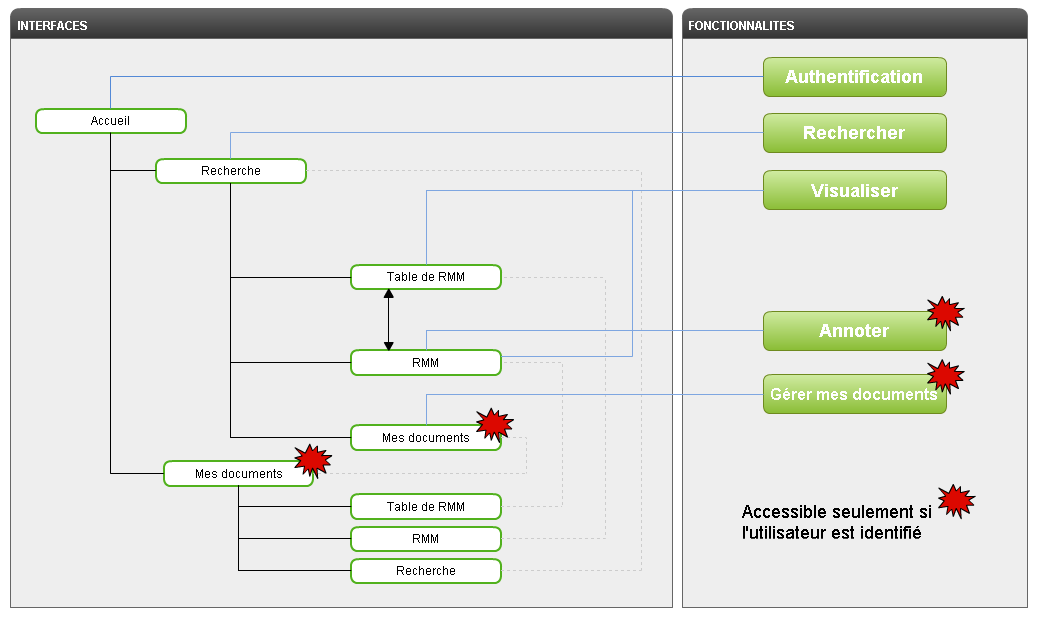
\includegraphics[width=\textwidth]{navigation.png}
\caption{Schéma de navigation de l'application}
\label{fig:navigation}
\end{figure}

Lorsque l’utilisateur commencera à utiliser l’application, celui-ci se retrouvera sur un écran d’accueil qui lui proposera deux fonctionnalités : s'inscrire ou bien s’identifier. Aussi, les écrans de recherche et de gestion devront être accessibles à partir de n’importe quel autre écran, hormis le cas particulier pour la gestion des documents. Elle sera accessible à partir de l’écran d’accueil seulement si l’utilisateur est déjà identifié. Les écrans de visualisation de document pourront être accessible à partir d’une recherche ou bien lorsque l’utilisateur souhaite consulter un de ses documents. Aussi, à partir d’une visualisation de table, il sera possible à l’utilisateur d’accéder à un ou plusieurs RMM.

\newpage
\section{Spécifications fonctionnelles du système}

\subsection{Authentification}

Un utilisateur, souhaitant simplement consulter les tables et les RMM, n'est pas obligé de s'authentifier. Cependant, si celui-ci souhaite bénéficier des outils d'annotation et de favoris, il devra impérativement s'authentifié. En effet, les annotations sont associées à un utilisateur, ce qui permettra, par la suite, de faciliter la modération.

\subsubsection{Page d'accueil} 

La page d'accueil est la première page que les utilisateurs verront. C'est pourquoi, cette page devra contenir les accès à toutes les fonctionnalités principales de notre application. Parmi ces fonctionnalités se trouvent celles liées à l'authentification. L'inscription à notre système se fera depuis l'écran d'accueil alors que la connexion pourra se faire quelque soit la page que l'utilisateur visualise. La figure \ref{fig:accueil} illustre l'écran d'accueil que pourra voir un utilisateur ne s'étant pas authentifié.

\begin{figure}[H]
\centering
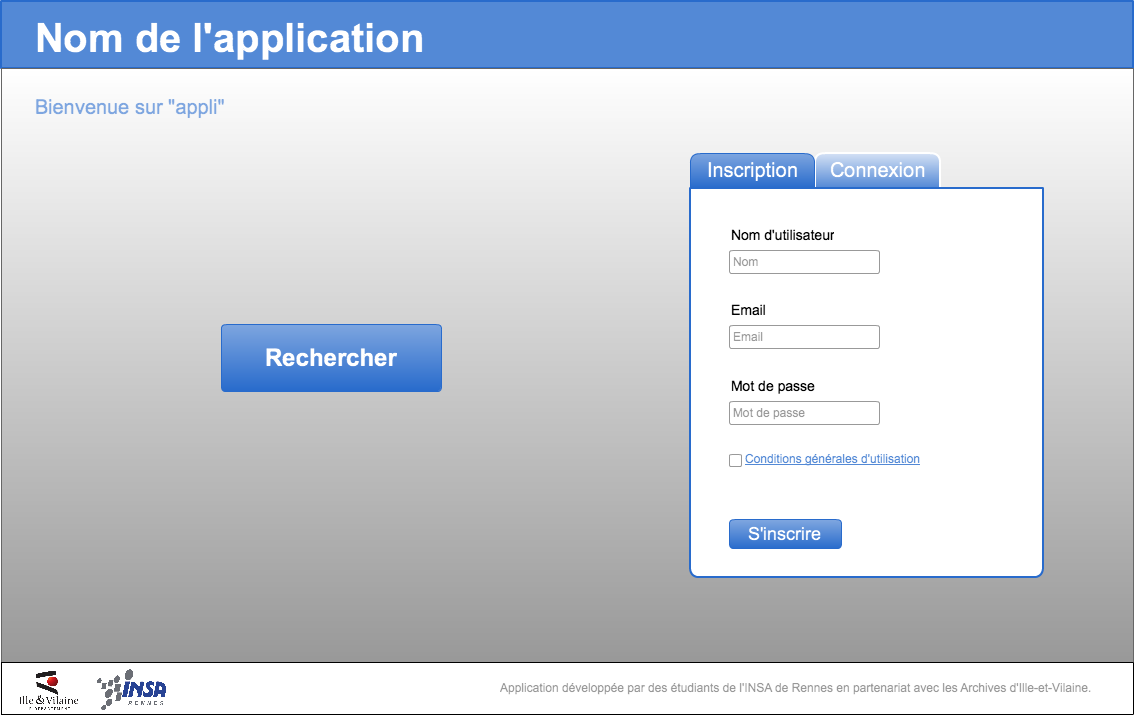
\includegraphics[width=\textwidth]{accueil.png}
\caption{Ecran d'accueil de notre application sur PixelSense}
\label{fig:accueil}
\end{figure}

\subsubsection{Fonction SA01 - Inscription}

L’inscription permet à l’utilisateur de s’enregistrer pour accéder à l’ensemble des fonctionnalités de l’application (pour visualiser ou annoter n’importe quel document). Il devra rentrer diverses informations; un identifiant, un mot de passe ainsi qu’un e-mail valide qui seront stockés sur la base de données prévue pour l’application. Par la suite, ses informations lui seront utiles pour s’identifier sur l’application afin qu’il accède à ses propres données dans le but qu’il puisse les gérer (ajouter une annotation, la modifier ou la supprimer).
    
\begin{table}[H]
  \centering
   \small
	\begin{tabular}{|c|p{12cm}|}
   		\hline
   			\rowcolor{lightgray}\multicolumn{2}{|c|}{\textbf{Fonction SA01 - Inscription}} \\
   		\hline
   			\multicolumn{2}{|l|}{Condition de déclenchement} \\
   		\hline
   			-1 & Un utilisateur non identifié veut s'inscrire à l'application.\\
   		\hline
   			\multicolumn{2}{|l|}{Déclenchement de l'opération} \\
   		\hline
   			-1 & L'utilisateur confirme son inscription et a rempli les informations demandées.\\
   		\hline
   			\multicolumn{2}{|l|}{Entrants de l'opération} \\
   		\hline
   			-1 & Un identifiant\\
        	-2 & Un mot de passe\\ 
        	-3 & Une adresse e-mail\\ 
   		\hline
   			\multicolumn{2}{|l|}{Traitement de l'opération} \\
  		\hline
   			-1 & Vérification de l'unicité de l'identifiant et de l'adresse e-mail dans la base de données.\\
        	-2 & Ajout de l'utilisateur (ses informations identifiant, mot de passe et e-mail) dans la base de données si succès de la vérification.\\
        	-3 & Refus de l'utilisateur si échec de la vérification.\\
   		\hline
   			\multicolumn{2}{|l|}{Sortants de l'opération} \\
   		\hline
   			-1 & Envoi d'une demande de confirmation sur l'e-mail indiqué si succès.\\
            -2 & Renvoi d'un nouveau formulaire d'inscription si échec.\\
   		\hline
	\end{tabular}
  \caption{Fonction SA01 - Inscription}
  \normalsize
  \label{tab: inscription}
\end{table}
    
    
\subsubsection{Fonction SA02 - Connexion}

La connexion permet à l’utilisateur de s’identifier pour accéder à l’ensemble des fonctionnalités de l’application. Pour ce faire, il devra compléter son identifiant et son mot de passe. Si ces informations se révèlent être correctes, l’utilisateur peut accéder à ses anciennes annotations, les modifier, les supprimer ou il peut annoter de nouveaux documents.

\begin{table}[H]
  \centering
   \small
	\begin{tabular}{|c|p{12cm}|}
   		\hline
   			\rowcolor{lightgray}\multicolumn{2}{|c|}{\textbf{Fonction SA02 - Connexion}} \\
   		\hline
   			\multicolumn{2}{|l|}{Condition de déclenchement} \\
   		\hline
   			-1 & Un utilisateur non identifié veut s'identifier\\
   		\hline
   			\multicolumn{2}{|l|}{Déclenchement de l'opération} \\
   		\hline
   			-1 & L'utilisateur demande à se connecter, complète les informations demandées puis valide.\\
   		\hline
   			\multicolumn{2}{|l|}{Entrants de l'opération} \\
   		\hline
   			-1 & Un identifiant\\
        	-2 & Un mot de passe\\
   		\hline
   			\multicolumn{2}{|l|}{Traitement de l'opération} \\
  		\hline
   			-1 & Vérification de l’existence de l'utilisateur dans la base de données.\\
        	-2 & Chargement des données de l'utilisateur si succès de la vérification.\\
        	-3 & Refus de la connexion si échec de la vérification.\\
   		\hline
   			\multicolumn{2}{|l|}{Sortants de l'opération} \\
   		\hline
   			-1 & Renvoi vers la page précédant la connexion si succès.\\
            -2 & Renvoi d'un nouveau formulaire de connexion si échec.\\
   		\hline
	\end{tabular}
  \caption{Fonction SA02 - Connexion}
  \normalsize
  \label{tab: connexion}
\end{table}

\subsubsection{Statuts des utilisateurs}

Un utilisateur n'a pas besoin d'être authentifié pour utiliser notre système. Cependant l'authentification permet à l'utilisateur d'accéder à des fonctionnalités supplémentaires. Aussi, nous allons retrouver plusieurs statuts parmi les utilisateurs authentifiés. La table \ref{tab:profils} résume les différents statuts avec les droits qui leur sont associés. 

\begin{table}[H]
	\centering
		\small
			\begin{tabular}{|c|p{7cm}|}
				\hline
					\rowcolor{lightgray}\textbf{Statut} & \textbf{Droits} \\
				\hline
					Utilisateur non-connecté & Rechercher un document, naviguer dans les documents, visualiser un document avec ses annotations \\
				\hline
					Utilisateur basique & Droits d'un utilisateur non-connecté, annoter un document, visualiser les annotations d'un autre utilisateur pour un document donné, utilisation de favoris \\
				\hline
					Modérateur & Droits d'un utilisateur non-connecté, supprimer un utilisateur basique\\
				\hline
					Administrateur & Droits d'un modérateur, supprimer un modérateur, supprimer un administrateur, modifier le statut d'un utilisateur \\
				\hline
			\end{tabular}
			\caption{Profils des utilisateurs}
		\normalsize
	\label{tab:profils}
\end{table}


\subsection{Navigation entre les documents}

La navigation est l'un des éléments indispensables de notre projet. En effet, il est impossible d'annoter des documents si on ne posssède pas la capacité de les parcourir. Les fonctionnalités que nous avons l'intention de dvelopper nous semblent être un bon compromis, afin d'éviter d'avoir une navigation trop simpliste, ou au contraire une navigation avec trop d'options, qui deviendrait ainsi laborieuse. 

\subsubsection{Navigation dans une table}

La table est l'un des deux documents de base de notre projet. En effet, même si la finalité des utilisateurs de notre solution est d'annoter des registres, la manière la plus intuitive d'accéder à ces registres est de passer par les tables. C'est pour celà que nous devons proposer une solution de navigation simple et intuitive au sein de tables.

\subsubsection{Fonction SB01 - Naviguer dans une m\^eme table jusqu'à une page adjacente}

La table est un ensemble de pages, qui recensent chacunes des dizaines d'individus. Ici, le but est simpement de permettre une navigation rapide entre des pages adjacentes (page suivante ou page pr\'ec\'edente).

Raccourci mouvement : L'utilisateur fait glisser son doigt de gauche \`a droite pour aller \`a l'image pr\'ec\'edente, ou de droite \`a gauche pour aller \`a la suivante.

\begin{table}[H]
  \centering
   \small
	\begin{tabular}{|c|p{12cm}|}
   		\hline
   			\rowcolor{lightgray}\multicolumn{2}{|c|}{\textbf{SB01 - Naviguer dans une m\^eme table jusqu'à une page adjacente}} \\
   		\hline
   			\multicolumn{2}{|l|}{Condition de d\'eclenchement} \\
   		\hline
   		-1 & Un utilisateur veut acc\'eder \`a une page adjacente de la table. \\
   		\hline
   			\multicolumn{2}{|l|}{D\'eclenchement de l'op\'eration} \\
   		\hline
   			-1 & L'utilisateur effectue le raccourci mouvement puis rel\^ache. \\
   		\hline
   			\multicolumn{2}{|l|}{Entrants de l'op\'eration} \\
   		\hline
   			-1 & Une page de la table \\
        	-2 & Un sens de d\'eplacement \\ 
   		\hline
   			\multicolumn{2}{|l|}{Traitement de l'op\'eration} \\
  		\hline
   			-1 & Associer une page au couple \{page actuelle, sens de d\'eplacement\}.  \\
        	-2 & V\'erifier que la page demand\'ee existe. \\
        	-3 & Afficher la page demand\'ee et la d\'efinir comme page actuelle. \\
   		\hline
   			\multicolumn{2}{|l|}{Sortants de l'op\'eration} \\
   		\hline
   			-1 & Affichage de la page demand\'ee. \\
   		\hline
	\end{tabular}
  \caption{SB01 - Naviguer dans une table}
  \normalsize
  \label{tab:naviguer_table_unique_adjacent}
\end{table}

\subsubsection{Fonction SB02 - Naviguer dans une m\^eme table jusqu'à une page numérotée}

Afin de navguer facilement dans les tables, la navigation vers les pages adjacentes ne suffit pas. En effet, si l'utilisateur veut atteindre une page éloigné de la page courante, par exemple la 20ème page en partant du début de la table, il  ne doit pas être obligé de répéter 20 fois l'action "aller à la page suivante". Cette fonctionnalité son numéro.  de sélectionner la page qu'on désire atteindre, en renseignant simplement
\begin{table}[H]
  \centering
   \small
	\begin{tabular}{|c|p{12cm}|}
   		\hline
   			\rowcolor{lightgray}\multicolumn{2}{|c|}{\textbf{SB02 - Naviguer dans une m\^eme table jusqu'à une page numérotée}} \\
   		\hline
   			\multicolumn{2}{|l|}{Condition de d\'eclenchement} \\
   		\hline
   		-1 & Un utilisateur veut acc\'eder \`a une page de la table. \\
   		\hline
   			\multicolumn{2}{|l|}{D\'eclenchement de l'op\'eration} \\
   		\hline
   			-1 & L'utilisateur entre le numéro de la page à atteindre et valide. \\
   		\hline
   			\multicolumn{2}{|l|}{Entrants de l'op\'eration} \\
   		\hline
   			-1 & La table courante. \\
        	-2 & Le numéro de la page à atteindre. \\ 
   		\hline
   			\multicolumn{2}{|l|}{Traitement de l'op\'eration} \\
  		\hline
   			-1 & Associer une page au couple \{table, numéro de page\}.  \\
        	-2 & V\'erifier que la page demand\'ee existe. \\
        	-3 & Afficher la page demand\'ee et la d\'efinir comme page actuelle. \\
   		\hline
   			\multicolumn{2}{|l|}{Sortants de l'op\'eration} \\
   		\hline
   			-1 & Affichage de la page demand\'ee. \\
   		\hline
	\end{tabular}
  \caption{SB02 - Naviguer dans une table jusqu'à une page numérotée}
  \normalsize
  \label{tab:naviguer_table_unique}
\end{table}


\subsubsection{Fonction SB03 - Naviguer entre deux tables}

Pour un utilisateur, il peut être intéressant de pouvoir naviguer rapidement de table en table, par exemple lorsqu'il recherche une personne dont il connaït le nom mais pas l'année d'entrée eb service. Dans ce cas, il va établir une fourchette contenant les années qu'il estime possibles, et parcourir les tables correspondant à ces années. Les tables seront classées par ordre chronologique (une par année), ainsi navuguer vers l'année suivante reviendra à naviguer vers la table suivante.

De plus, si on cherche un nom précis, il est fastidieux de devoir, pour chaque table, trouver la page correspondant au nom de l'individu (clasés par ordre alphabétique). C'est pourquoi il paraît utile de proposer à l'utilisateur de naviguer vers une autre année, tout en essayant d'atteindre directement la page qui l'intéresse. En partant du principe que la distribution des noms de famille alphabétiquement parlant est à peu près identique d'une année sur l'autre, on peut ainsi définir une fontion proportionnelle. Par exeple, en étant à la page 6/30 de la table de l'année N, on se retrouvera à la page 4/20 de l'année N+1.

\begin{table}[H]
  \centering
   \small
	\begin{tabular}{|c|p{12cm}|}
   		\hline
   			\rowcolor{lightgray}\multicolumn{2}{|c|}{\textbf{SB03 - Naviguer entre deux tables}} \\
   		\hline
   			\multicolumn{2}{|l|}{Condition de d\'eclenchement} \\
   		\hline
   		-1 & Un utilisateur veut acc\'eder \`a une table adjacente à la table actuelle. \\
   		\hline
   			\multicolumn{2}{|l|}{D\'eclenchement de l'op\'eration} \\
   		\hline
   			-1 & L'utilisateur clique sur le bouton correspondant. \\
   		\hline
   			\multicolumn{2}{|l|}{Entrants de l'op\'eration} \\
   		\hline
   			-1 & Une page de la table \\
        	-2 & Le nombre de pages de la table \\ 
            -3 & Le sens de déplacement (année suivante ou précédente). \\
   		\hline
   			\multicolumn{2}{|l|}{Traitement de l'op\'eration} \\
  		\hline
   			-1 & Associer une table au couple \{table actuelle, sens de d\'eplacement\}.  \\
        	-2 & V\'erifier que la table demand\'ee existe. \\
        	-3 & Déterminer la page à atteindre en fonction du ratio \{numéro de page/nombre de page\} de la page de départ et du nombre de pages de la table à atteindre. \\
            -4 & Afficher la table visée à la bonne page. \\
   		\hline
   			\multicolumn{2}{|l|}{Sortants de l'op\'eration} \\
   		\hline
   			-1 & Affichage de la table demand\'ee. \\
   		\hline
	\end{tabular}
  \caption{SB03 - Naviguer entre deux tables}
  \normalsize
  \label{tab:naviguer_deux_tables}
\end{table}


\subsubsection{Naviguer entre deux RMM}

Même si la navigation au sein des tables est primordiale, il ne faut pas négliger la possibilité que certains utilisateurs annotent des registres "à la chaîne", parfois sans même passer par les tables. Il faut donc que notre solution propose aussi une solution de navigation entre les registres.

\subsubsection{Fonction SB04 - Naviguer entre deux RMM adjacents}

Pour certains utilisateurs, qui annotent de nombreux RMM quasiment "à la chaîne", la fonctionnalité de navigation entre des RMM adjacents est indispensable. Cette navigation entre deux RMM sera très proche de la navigation entre deux pages adjacentes d'une table.

Raccourci mouvement : Identique à celui de la navigation entre pages adjacentes d'une table. L'utilisateur fait glisser son doigt de gauche \`a droite pour aller \`a l'image pr\'ec\'edente, ou de droite \`a gauche pour aller \`a la suivante.

\begin{table}[H]
  \centering
   \small
	\begin{tabular}{|c|p{12cm}|}
   		\hline
   			\rowcolor{lightgray}\multicolumn{2}{|c|}{\textbf{SB04 - Naviguer entre deux RMM adjacents}} \\
   		\hline
   			\multicolumn{2}{|l|}{Condition de d\'eclenchement} \\
   		\hline
   		-1 & Un utilisateur veut acc\'eder \`a un RMM adjacent au RMM actuel. \\
   		\hline
   			\multicolumn{2}{|l|}{D\'eclenchement de l'op\'eration} \\
   		\hline
   			-1 & L'utilisateur effectue le raccourci mouvement puis rel\^ache. \\
   		\hline
   			\multicolumn{2}{|l|}{Entrants de l'op\'eration} \\
   		\hline
   			-1 & Un RMM \\
        	-2 & Un sens de d\'eplacement \\ 
   		\hline
   			\multicolumn{2}{|l|}{Traitement de l'op\'eration} \\
  		\hline
   			-1 & Associer un RMM au couple \{RMM actuel, sens de d\'eplacement\}.  \\
        	-2 & V\'erifier que le RMM demand\'e existe. \\
        	-3 & Afficher le RMM demand\'e et le d\'efinir comme registre actuel. \\
   		\hline
   			\multicolumn{2}{|l|}{Sortants de l'op\'eration} \\
   		\hline
   			-1 & Affichage du RMM demand\'e. \\
   		\hline
	\end{tabular}
  \caption{SB04 - Naviguer entre deux RMM}
  \normalsize
  \label{tab:naviguer_deux_registres_adjacents}
\end{table}

\subsubsection{Fonction SB05 - Naviguer entre deux RMM numérotés}

Dans notre base d'images de RMM, celles-ci sont classées par numéros de matricule. Cependant, à cause des vues multiples dues aux retombes et aux éventuelles absences de certains RMM, numéro de matricule et numéro d'image ne correspondent pas forcément. Cependant, certains utilisateurs peuvent vouloir accéder rapidement à un RMM en ne connaissant que le numéro de l'image, par exemple sur les conseils d'un ami. Ainsi, en entrant le numéro souhaité, on accède directement à l'image correspondante.

\begin{table}[H]
  \centering
   \small
  \begin{tabular}{|c|p{12cm}|}
      \hline
        \rowcolor{lightgray}\multicolumn{2}{|c|}{\textbf{SB05 - Naviguer entre deux RMM numérotés}} \\
      \hline
        \multicolumn{2}{|l|}{Condition de d\'eclenchement} \\
      \hline
      -1 & Un utilisateur veut acc\'eder \`a un RMM via son numéro. \\
      \hline
        \multicolumn{2}{|l|}{D\'eclenchement de l'op\'eration} \\
      \hline
        -1 & L'utilisateur indique le numéro de l'image souhaitée. \\
      \hline
        \multicolumn{2}{|l|}{Entrants de l'op\'eration} \\
      \hline
        -1 & Un dossier d'image \\
          -2 & Un numéro d'image \\ 
      \hline
        \multicolumn{2}{|l|}{Traitement de l'op\'eration} \\
      \hline
        -1 & Associer une image au couple \{dossier d'images actuel, numéro d'image\}.  \\
          -2 & V\'erifier que l'image' demand\'ee existe. \\
          -3 & Afficher l'image' demand\'ee et définir le RMM comme RMM actuel. \\
      \hline
        \multicolumn{2}{|l|}{Sortants de l'op\'eration} \\
      \hline
        -1 & Affichage de l'image demand\'ee. \\
      \hline
  \end{tabular}
  \caption{SB05 - Naviguer entre deux RMM numérotés}
  \normalsize
  \label{tab:naviguer_deux_registres_numerotes}
\end{table}


\subsubsection{Naviguer d'une table à un RMM}

Lorsqu'un uilisateur recherche un individu dont il connaît le nom et la date d'engagement, la méthode d'accès la plus intuitive est de trouver cet individu dans la table correspondante, afin de récupérer son numéro matricule et ainsi de le retrouver dans les registres. Afin d'éviter à l'utilisateur des allers-retours entre ces différents types de documents, nous allons proposer une fonctionnalité qui fera directement le lien entre une table et un RMM.

Pour cela, l'utilisateur devra simplement annoter le numéro de matricule de l'individu qui l'intéresse dans la table (et éventuellement ses nom/prénoms), puis le système se chargera de trouver le registre demandé. Il y a deux cas de figure : où un autre utilisateur a déjà lié ce numéro de matricule à un RMM, auquel cas on renvoie ce registre. Dans l'autre cas, si on ne peut lier le numéro de matricule à un RMM, alors on lance une recherche sur le numéro de matricule. 

\subsubsection{Fonction SB06 - Naviguer d'une table à un RMM inconnu}

Ici, on se place dans le cas où le numéro de matricule ne permet pas de trouver le RMM correspondant, c'est à dire que ce dernier n'a pas été annoté. 

\begin{table}[H]
  \centering
   \small
	\begin{tabular}{|c|p{12cm}|}
   		\hline
   			\rowcolor{lightgray}\multicolumn{2}{|c|}{\textbf{SB06 - Naviguer d'une table à un RMM inconnu}} \\
   		\hline
   			\multicolumn{2}{|l|}{Condition de d\'eclenchement} \\
   		\hline
   			-1 & Un utilisateur veut acc\'eder \`a un registre à partir d'une table. \\
   		\hline
   			\multicolumn{2}{|l|}{D\'eclenchement de l'op\'eration} \\
   		\hline
   			-1 & L'utilisateur clique dans la table sur la ligne de l'individu qui l'intéresse, puis annote son numéro de matricule. \\
   		\hline
   			\multicolumn{2}{|l|}{Entrants de l'op\'eration} \\
   		\hline
   			-1 & Une table \\
        			-2 & Un numéro de registre \\ 
   		\hline
   			\multicolumn{2}{|l|}{Traitement de l'op\'eration} \\
  		\hline
   			-1 & Associer une requête de recherche au couple \{année de la table, numéro de registre\} \\
   		\hline
   			\multicolumn{2}{|l|}{Sortants de l'op\'eration} \\
   		\hline
   			-1 & Renvoi et traitement de la recherche \\
   		\hline
	\end{tabular}
  \caption{SB06 - Naviguer d'une table à un RMM inconnu}
  \normalsize
  \label{tab:naviguer_table_registre_inconnu}
\end{table}



\subsubsection{Fonction SB07 - Naviguer d'une table à un RMM connu}

Ici, on se place dans le cas où le numéro de matricule permet de trouver le RMM correspondant, car ce dernier a déjà été annoté.

\begin{table}[H]
  \centering
   \small
  \begin{tabular}{|c|p{12cm}|}
      \hline
        \rowcolor{lightgray}\multicolumn{2}{|c|}{\textbf{SB07 - Naviguer d'une table à un RMM connu}} \\
      \hline
        \multicolumn{2}{|l|}{Condition de d\'eclenchement} \\
      \hline
      -1 & Un utilisateur veut acc\'eder \`a un registre à partir d'une table. \\
      \hline
        \multicolumn{2}{|l|}{D\'eclenchement de l'op\'eration} \\
      \hline
        -1 & L'utilisateur clique dans la table sur la ligne de l'individu qui l'intéresse, puis annote son numéro de matricule. \\
      \hline
        \multicolumn{2}{|l|}{Entrants de l'op\'eration} \\
      \hline
        -1 & Une table \\
          -2 & Un numéro de registre \\ 
      \hline
        \multicolumn{2}{|l|}{Traitement de l'op\'eration} \\
      \hline
        -1 & Trouver le registre correspondant au couple \{numéro de matricule, année de la table\} \\
          -2 & Afficher le registre correspondant. \\
      \hline
        \multicolumn{2}{|l|}{Sortants de l'op\'eration} \\
      \hline
        -1 & Affichage du registre demand\'e \\
      \hline
  \end{tabular}
  \caption{SB07 - Naviguer d'une table à un RMM connu}
  \normalsize
  \label{tab:naviguer_table_registre_connu}
\end{table}


\subsection{Annotation}

	Une annotation est caractérisée par 3 attributs : sa position sur le RMM, sa catégorie et son texte. Par exemple, si on veut annoter la nom d’un RMM, cette annotation aura pour catégorie « Nom » et pour texte le nom de la personne et se situera au niveau de son nom sur le RMM. Les catégories ne seront pas libres, l’utilisateur pourra seulement sélectionner la catégorie parmi une liste de catégorie.

\subsubsection{Fonction SC01 - Annoter une table}


L'annotation de table permet de cr\'eer un lien avec les registres. En annotant le num\'ero de matricule et le nom associ\'e, on cr\'e\'e un pivot. Ce pivot peut \^etre temporaire si le registre associ\'e n'a pas \'et\'e annot\'e, sinon le pivot est valide (registre annot\'e).\\

\begin{table}[H]
  \centering
   \small
	\begin{tabular}{|c|p{12cm}|}
   		\hline
   			\rowcolor{lightgray}\multicolumn{2}{|c|}{\textbf{SC01 - Annoter une table}} \\
   		\hline
   			\multicolumn{2}{|l|}{Condition de d\'eclenchement} \\
   		\hline
   		-1 & Un utilisateur veut annoter une ligne d'une table. \\
   		\hline
   			\multicolumn{2}{|l|}{D\'eclenchement de l'op\'eration} \\
   		\hline
   			-1 & L'utilisateur clique sur le bouton correspondant. \\
   		\hline
   			\multicolumn{2}{|l|}{Entrants de l'op\'eration} \\
   		\hline
   			-1 & Nom et pr\'enoms \\
        	-2 & Num\'ero de matricule \\ 
        	-3 & Zone de d\'elimitation de l'annotation (rectangle) \\
            -4 & Liste des annotations d\'ej\`a associ\'ees \`a cette ligne \\
   		\hline
   			\multicolumn{2}{|l|}{Traitement de l'op\'eration} \\
  		\hline
   			-1 & Ajout dans la base de donn\'ees. \\
        	-2 & V\'erifier si une annotation correspond d\'ej\`a \`a cette ligne \\
        	-3 & Cr\'eation d'un pivot \\
            -4 & Ajout du document annot\'e dans le dossier mes annotations. \\
   		\hline
   			\multicolumn{2}{|l|}{Sortants de l'op\'eration} \\
   		\hline
   			-1 & Affichage de l'annotation. \\
            -2 & Pivot \\
   		\hline
	\end{tabular}
  \caption{SC01 - Annoter une table}
  \normalsize
  \label{tab:annoter_table}
\end{table}

\subsubsection{Fonction SC02 - Annoter un RMM}

Un utilisateur visualise un RMM et souhaite annoter son contenu. Pour faire cela il doit appuyer à l’endroit où il souhaite annoter, ce qui va permettre de créer une annotation avec sa position sur l’image. Une catégorie d’annotation sera suggérée. Si l’utilisateur veut créer une annotation sans catégorie particulière, il peut choisir la catégorie « Autre catégorie ». Il doit ensuite remplir le texte de l’annotation et la valider. Les annotations faites sur un RMM met à jour la fiche d’identité associé au RMM. Elle sera ensuite enregistrée sur la base de données.\\

\begin{table}[H]
  \centering
   \small
	\begin{tabular}{|c|p{12cm}|}
   		\hline
   			\rowcolor{lightgray}\multicolumn{2}{|c|}{\textbf{SC02 - Annoter un RMM}} \\
   		\hline
   			\multicolumn{2}{|l|}{Condition de d\'eclenchement} \\
   		\hline
   			-1 & L'utilisateur visualise un RMM et est connecté\\
   		\hline
   			\multicolumn{2}{|l|}{D\'eclenchement de l'op\'eration} \\
   		\hline
   			-1 & L’utilisateur clique sur ce qu’il souhaite annoter sur l’image\\
   		\hline
   			\multicolumn{2}{|l|}{Entrants de l'op\'eration} \\
   		\hline
   			-1 & Détection possible du type de l’annotation en fonction de la position de l'annotation afin de pré-remplir la catégorie d’annotation\\
            -2 & Choix de la catégorie de l’annotation \\
			-3 & Choix du texte de l’annotation obligatoire \\
   		\hline
   			\multicolumn{2}{|l|}{Traitement de l'op\'eration} \\
  		\hline
   			-1 & Sauvegarde de l’annotation dans la base de données\\
   		\hline
   			\multicolumn{2}{|l|}{Sortants de l'op\'eration} \\
   		\hline
   			-1 & Ajoute l’annotation à la liste des annotations du document (elle va apparaitre dans la fiche d’identité du RMM\\
			-2 & Visualisation de l’image\\
   		\hline
	\end{tabular}
  \caption{SC02 - Annoter un RMM}
  \normalsize
  \label{tab:annoter_registre}
\end{table}

\subsubsection{Fonction SC03 - Annoter un RMM en cliquant sur la fiche identité}
Une deuxième façon d’annoter un RMM est d’utiliser des annotations pré-remplie en cliquant sur l’annotation voulue au niveau de la fiche d’identité.\\

\begin{table}[H]
  \centering
   \small
	\begin{tabular}{|c|p{12cm}|}
   		\hline
   			\rowcolor{lightgray}\multicolumn{2}{|c|}{\textbf{SC03 -  Annoter un RMM en cliquant sur la fiche identité}} \\
   		\hline
   			\multicolumn{2}{|l|}{Condition de d\'eclenchement} \\
   		\hline
   		-1 & L'utilisateur visualise un RMM et est connecté\\
   		\hline
   			\multicolumn{2}{|l|}{D\'eclenchement de l'op\'eration} \\
   		\hline
   			-1 & L’utilisateur clique sur ce qu’il souhaite annoter au niveau de la fiche d’identité\\
   		\hline
   			\multicolumn{2}{|l|}{Entrants de l'op\'eration} \\
   		\hline
        	-1 & Choix du texte de l’annotation obligatoire\\
   		\hline
   			\multicolumn{2}{|l|}{Traitement de l'op\'eration} \\
  		\hline
   			-1 & Sauvegarde de l’annotation dans la base de données\\

   		\hline
   			\multicolumn{2}{|l|}{Sortants de l'op\'eration} \\
   		\hline
   			-1 & Ajoute l’annotation à la liste des annotations du document, elle va apparaitre dans
la fiche d’identité du RMM\\
   		\hline
	\end{tabular}
  \caption{SC03 - Annoter un RMM en cliquant sur la fiche identité}
  \normalsize
  \label{tab:annotation_fiche}
\end{table}

\subsubsection{Fonction SC04 - Annoter grâce à un raccourci}
L’utilisateur souhaite utiliser un raccourci pour annoter une image. Pour cela il doit déplacer un bouton raccourci à l’endroit voulu, ce qui permet de créer une annotation à cet endroit avec une catégorie prédéfinie par ce raccourci.\\

\begin{table}[H]
  \centering
   \small
	\begin{tabular}{|c|p{12cm}|}
   		\hline
   			\rowcolor{lightgray}\multicolumn{2}{|c|}{\textbf{SC04 - Annoter grâce à un raccourci}} \\
   		\hline
   			\multicolumn{2}{|l|}{Condition de d\'eclenchement} \\
   		\hline
   			-1 & L’utilisateur souhaite utiliser un raccourci pour annoter une image\\
   		\hline
   			\multicolumn{2}{|l|}{D\'eclenchement de l'op\'eration} \\
   		\hline
   			-1 & L’utilisateur commence à appuyer sur un raccourci\\
   		\hline
   			\multicolumn{2}{|l|}{Entrants de l'op\'eration} \\
   		\hline
   			-1 & L’utilisateur place le raccourci à l’endroit voulu\\
			-2 & Fait apparaitre une fenêtre avec la catégorie déjà remplie\\
			-3 & L’utilisateur rentre le texte de l’annotation\\
			-4 & L’utilisateur valide l’annotation\\
   		\hline
   			\multicolumn{2}{|l|}{Traitement de l'op\'eration} \\
  		\hline
   			-1 & Sauvegarde l’annotation dans la base de données\\
   		\hline
   			\multicolumn{2}{|l|}{Sortants de l'op\'eration} \\
   		\hline
   			-1 & Ajoute l’annotation à la liste des annotations du document elle va apparaitre dans la fiche d’identité du RMM\\
   		\hline
	\end{tabular}
  \caption{SC04 - Annoter grâce à un raccourci}
  \normalsize
  \label{tab:utiliser_raccourci}
\end{table}

\subsubsection{Fonction SC05 - Affichage d'une fiche d'identité d'un soldat}

Le but de la fiche d'identité d'un soldat est d'exploiter au maximum les annotations d'un registre. Gr\^ace aux cat\'egories, il est possible de g\'en\'erer automatiquement une fiche avec toutes les informations importantes. De plus, cette fiche va servir de checklist des annotations \`a faire et pouvant \^etre faite.\\

\begin{table}[H]
  \centering
   \small
	\begin{tabular}{|c|p{12cm}|}
   		\hline
   			\rowcolor{lightgray}\multicolumn{2}{|c|}{\textbf{SC05 - Affichage d'une fiche d'identité d'un soldat}} \\
   		\hline
   			\multicolumn{2}{|l|}{Condition de d\'eclenchement} \\
   		\hline
   		-1 & Un utilisateur consulte un registre, la fiche soldat est affich\'ee en m\^eme temps. \\
   		\hline
   			\multicolumn{2}{|l|}{D\'eclenchement de l'op\'eration} \\
   		\hline
   			-1 & L'utilisateur navigue sur un registre. \\
   		\hline
   			\multicolumn{2}{|l|}{Entrants de l'op\'eration} \\
   		\hline
   			-1 & Registre \\
   		\hline
   			\multicolumn{2}{|l|}{Traitement de l'op\'eration} \\
  		\hline
   			-1 & Recherche dans la base de donn\'ees \\
            -2 & G\'en\'eration de la fiche \\
   		\hline
   			\multicolumn{2}{|l|}{Sortants de l'op\'eration} \\
   		\hline
   			-1 & Affichage de la fiche. \\
   		\hline
	\end{tabular}
  \caption{SC05 - Affichage d'une fiche d'identité d'un soldat}
  \normalsize
  \label{tab:affichage_fiche}
\end{table}


\subsubsection{Fonction SC06 - Afficher les positions de toutes les annotations}
Les annotations apparaissent à droite de l’écran lorsque l’on visualise une image. Cliquer sur la case à cocher en haut à droite de l’interface permet d’afficher ou de masquer les annotations. Ces positions sont représentées par des points sur le document.\\

\begin{table}[H]
  \centering
   \small
	\begin{tabular}{|c|p{12cm}|}
   		\hline
   			\rowcolor{lightgray}\multicolumn{2}{|c|}{\textbf{SC06 - Afficher les positions de toutes les annotations}} \\
   		\hline
   			\multicolumn{2}{|l|}{Condition de d\'eclenchement} \\
   		\hline
   			-1 & Un utilisateur visualise un RMM et les annotations sont masquées\\
   		\hline
   			\multicolumn{2}{|l|}{D\'eclenchement de l'op\'eration} \\
   		\hline
   			-1 & L’utilisateur clique sur la case à cocher\\
   		\hline
   			\multicolumn{2}{|l|}{Entrants de l'op\'eration} \\
   		\hline
   			-1 & L’utilisateur clique sur la case à cocher\\
   		\hline
   			\multicolumn{2}{|l|}{Traitement de l'op\'eration} \\
  		\hline
   			-1 & Fait apparaitre la position de chaque annotation\\
   		\hline
   			\multicolumn{2}{|l|}{Sortants de l'op\'eration} \\
   		\hline
   			-1 & Visualisation de l’image et de ses annotations\\
   		\hline
	\end{tabular}
  \caption{SC06 - Afficher les positions de toutes les annotations}
  \normalsize
  \label{tab:visualiser_position_annotation}
\end{table}

\subsubsection{Fonction SC07 - Masquer les positions des annotations}
De la même manière la position des annotations peuvent être masquées.\\

\begin{table}[H]
  \centering
   \small
	\begin{tabular}{|c|p{12cm}|}
   		\hline
   			\rowcolor{lightgray}\multicolumn{2}{|c|}{\textbf{SC07 - Masquer les positions des annotations}} \\
   		\hline
   			\multicolumn{2}{|l|}{Condition de d\'eclenchement} \\
   		\hline
   			-1 & Un utilisateur visualise un RMM et les annotations sont visibles\\
   		\hline
   			\multicolumn{2}{|l|}{D\'eclenchement de l'op\'eration} \\
   		\hline
   			-1 & L’utilisateur clique sur la case à cocher\\
   		\hline
   			\multicolumn{2}{|l|}{Entrants de l'op\'eration} \\
   		\hline
   			-1 & L’utilisateur clique sur la case à cocher\\
   		\hline
   			\multicolumn{2}{|l|}{Traitement de l'op\'eration} \\
  		\hline
   			-1 & Masque la position de chaque annotation\\
   		\hline
   			\multicolumn{2}{|l|}{Sortants de l'op\'eration} \\
   		\hline
   			-1 & Visualisation de l’image\\
   		\hline
	\end{tabular}
  \caption{SC07 - Masquer les positions des annotations}
  \normalsize
  \label{tab:masquer_position_annotation}
\end{table}

\subsubsection{Fonction SC08 - Sélectionner une annotation sur un document}
Un utilisateur peut sélectionner une annotation. Cliquer sur une annotation au niveau de la fiche d’identité ou sur un point en particulier (si on a affiché les annotations) la sélectionne. Quand une annotation est sélectionnée, le point de la position de l’annotation est plus gros par rapport aux autres. On ne peut sélectionner qu’une seule annotation à la fois. C’est-à-dire que si on sélectionne une autre annotation, la précédente regagne se taille et la fenêtre disparait.\\

\begin{table}[H]
  \centering
   \small
	\begin{tabular}{|c|p{12cm}|}
   		\hline
   			\rowcolor{lightgray}\multicolumn{2}{|c|}{\textbf{SC08 - Sélectionner une annotation sur un document}} \\
   		\hline
   			\multicolumn{2}{|l|}{Condition de d\'eclenchement} \\
   		\hline
   			-1 & Un utilisateur veut visualiser la position d’une annotation en particulier\\
   		\hline
   			\multicolumn{2}{|l|}{D\'eclenchement de l'op\'eration} \\
   		\hline
   			-1 & Cliquer sur une annotation au niveau de la fiche d’identité\\
            -2 & Cliquer sur la position d'une annotation si on a affiché les annotations\\
   		\hline
   			\multicolumn{2}{|l|}{Entrants de l'op\'eration} \\
   		\hline
   			-1 & Cliquer sur une annotation au niveau de la fiche d’identité\\
            -2 & Cliquer sur la position d'une annotation\\
   		\hline
   			\multicolumn{2}{|l|}{Traitement de l'op\'eration} \\
  		\hline
   			-1 & Fait apparaitre la position de chaque annotation et coche la case associée\\
			-2 & Désélectionne l’ancienne annotation sélectionnée\\
			-3 & Fait apparaitre la position de l’annotation sélectionnée en plus gros\\
   		\hline
   			\multicolumn{2}{|l|}{Sortants de l'op\'eration} \\
   		\hline
   			-1 & Visualisation de l’image et de ses annotations\\
   		\hline
	\end{tabular}
  \caption{SC08 - Sélectionner une annotation sur un document}
  \normalsize
  \label{tab:selectionner_annotation}
\end{table}

\subsubsection{Fonction SC09 - Désélectionner une annotation sur un document}
Décocher la case associée à l’affichage permet de désélectionner une annotation tout en masquant celles-ci.\\

\begin{table}[H]
  \centering
   \small
	\begin{tabular}{|c|p{12cm}|}
   		\hline
   			\rowcolor{lightgray}\multicolumn{2}{|c|}{\textbf{SC09 - Désélectionner une annotation sur un document}} \\
   		\hline
   			\multicolumn{2}{|l|}{Condition de d\'eclenchement} \\
   		\hline
   			-1 & Un utilisateur veut désélectionner une annotation\\
   		\hline
   			\multicolumn{2}{|l|}{D\'eclenchement de l'op\'eration} \\
   		\hline
   			-1 & L’utilisateur masque les annotations\\
   		\hline
   			\multicolumn{2}{|l|}{Entrants de l'op\'eration} \\
   		\hline
   			-1 & L’utilisateur masque les annotations\\
   		\hline
   			\multicolumn{2}{|l|}{Traitement de l'op\'eration} \\
  		\hline
   			-1 & Désélectionne l’annotation\\
			-2 & Masque les annotations\\
   		\hline
   			\multicolumn{2}{|l|}{Sortants de l'op\'eration} \\
   		\hline
   			-1 & Visualisation de l’image\\
   		\hline
	\end{tabular}
  \caption{SC09 - Désélectionner une annotation sur un document}
  \normalsize
  \label{tab:deselectionner_annotation}
\end{table}

\subsubsection{Fonction SC10 - Modification de la position d’une annotation}
Après avoir sélectionné une annotation, un utilisateur qui possède cette annotation (c’est-à-dire qu’il l’a lui-même créée, ou qu’il l’a récupérée d’un autre utilisateur) peut modifier sa position.\\

\begin{table}[H]
  \centering
   \small
	\begin{tabular}{|c|p{12cm}|}
   		\hline
   			\rowcolor{lightgray}\multicolumn{2}{|c|}{\textbf{SC10 - Modification de la position d’une annotation}} \\
   		\hline
   			\multicolumn{2}{|l|}{Condition de d\'eclenchement} \\
   		\hline
   			-1 & L’utilisateur veut modifier la position d’une annotation\\
			-2 & L’utilisateur a sélectionné l’annotation\\
   		\hline
   			\multicolumn{2}{|l|}{D\'eclenchement de l'op\'eration} \\
   		\hline
   			-1 & L’utilisateur déplace l’annotation en maintenant son doigt appuyé\\
   		\hline
   			\multicolumn{2}{|l|}{Entrants de l'op\'eration} \\
   		\hline
   			-1 & L’utilisateur commence à déplacer l’annotation\\
   		\hline
   			\multicolumn{2}{|l|}{Traitement de l'op\'eration} \\
  		\hline
   			-1 & L’utilisateur relâche le point\\
			-2 & Modification de la position de l’annotation dans la base de données\\
   		\hline
   			\multicolumn{2}{|l|}{Sortants de l'op\'eration} \\
   		\hline
   			-1 & Visualisation de l’image et de ses annotations, avec sélection de l’annotation\\
   		\hline
	\end{tabular}
  \caption{SC10 - Modification de la position d’une annotation}
  \normalsize
  \label{tab:modification_position_annotation}
\end{table}

\subsubsection{Fonction SC11 - Modification du texte d’une annotation}
Après avoir sélectionné une annotation, un utilisateur qui possède cette annotation peut modifier son texte au niveau de la fiche d'indentité. Il est impossible de modifier la catégorie d'une annotation, l'utilisateur devra supprimer et recréer l'annotation s'il souhaite changer de catégorie.\\

\begin{table}[H]
  \centering
   \small
	\begin{tabular}{|c|p{12cm}|}
   		\hline
   			\rowcolor{lightgray}\multicolumn{2}{|c|}{\textbf{SC11 - Modification du champ d’une annotation}} \\
   		\hline
   			\multicolumn{2}{|l|}{Condition de d\'eclenchement} \\
   		\hline
   			-1 & L’utilisateur veut modifier le texte d'une annotation\\
			-2 & L’utilisateur a sélectionné cette annotation\\
   		\hline
   			\multicolumn{2}{|l|}{D\'eclenchement de l'op\'eration} \\
   		\hline
   			-1 & L’utilisateur commence à modifier un le texte de l'annotation au niveau de la fiche d'identité\\
   		\hline
   			\multicolumn{2}{|l|}{Entrants de l'op\'eration} \\
   		\hline
   			-1 & L’utilisateur modifie le texte de l'annotation\\
   		\hline
   			\multicolumn{2}{|l|}{Traitement de l'op\'eration} \\
  		\hline
   			-1 & L’utilisateur valide la modification\\
            -2 & Modification du texte de l'annotation dans la base de données\\
   		\hline
   			\multicolumn{2}{|l|}{Sortants de l'op\'eration} \\
   		\hline
   			-1 & Visualisation de l’image et de ses annotations, avec sélection de l’annotation\\
   		\hline
	\end{tabular}
  \caption{SC11 - Modification du champ d’une annotation}
  \normalsize
  \label{tab:modification_champ_annotation}
\end{table}

\subsubsection{Fonction SC12 - Suppression d'une annotation}
Après avoir sélectionné une annotation, un utilisateur qui possède cette annotation peut la supprimer.\\

\begin{table}[H]
  \centering
   \small
	\begin{tabular}{|c|p{12cm}|}
   		\hline
   			\rowcolor{lightgray}\multicolumn{2}{|c|}{\textbf{SC12 - Suppression d'une annotation}} \\
   		\hline
   			\multicolumn{2}{|l|}{Condition de d\'eclenchement} \\
   		\hline
   			-1 & L’utilisateur veut supprimer une annotation\\
			-2 & L’utilisateur a sélectionné l’annotation\\
   		\hline
   			\multicolumn{2}{|l|}{D\'eclenchement de l'op\'eration} \\
   		\hline
   			-1 & L’utilisateur déplace l’annotation vers une corbeille\\
			-2 & L’utilisateur clique sur Suppr ou sur un bouton supprimer\\
   		\hline
   			\multicolumn{2}{|l|}{Entrants de l'op\'eration} \\
   		\hline
   			-1 & L’utilisateur confirme la suppression\\
   		\hline
   			\multicolumn{2}{|l|}{Traitement de l'op\'eration} \\
  		\hline
   			-1 & Suppression de l’annotation dans la base de données\\
   		\hline
   			\multicolumn{2}{|l|}{Sortants de l'op\'eration} \\
   		\hline
   			-1 & Supprime l’annotation de la liste des annotations du document\\
			-2 & Visualisation de l’image et de ses annotations\\
   		\hline
	\end{tabular}
  \caption{SC12 - Suppression d'une annotation}
  \normalsize
  \label{tab:supprimer_annotation}
\end{table}

\subsubsection{Fonction SC13 - Consulter des fiches d’identités et en sélectionner une}
Un utilisateur peut consulter les fiches d’identités des autres utilisateurs, ce qui revient à visualiser des annotations déjà réalisées. Si la fiche est intéressante on peut la copier, c’est-à-dire s’approprier toutes les annotations. Pendant la sélection de la fiche on peut revenir à la visualisation du RMM précédant. Une fois la fiche copiée, on peut modifier ou supprimer les annotations.
La maquette suivant illustre l’interface permettant de sélectionner une fiche d’identité.\\

\begin{table}[H]
  \centering
   \small
	\begin{tabular}{|c|p{12cm}|}
   		\hline
   			\rowcolor{lightgray}\multicolumn{2}{|c|}{\textbf{SC13 - Consulter des fiches d’identités et en sélectionner une}} \\
   		\hline
   			\multicolumn{2}{|l|}{Condition de d\'eclenchement} \\
   		\hline
   			-1 & un utilisateur veut consulter les fiches d’identités pour en sélectionner une\\
   		\hline
   			\multicolumn{2}{|l|}{D\'eclenchement de l'op\'eration} \\
   		\hline
   			-1 & l’utilisateur clique sur « consulter fiche d’identité » et arrive sur l'interface de visualisation des fiches d'identités\\
   		\hline
   			\multicolumn{2}{|l|}{Entrants de l'op\'eration} \\
   		\hline
   			-1 & L’utilisateur visualise des fiches d’identités en les faisant défiler\\
			-2 & L'utilisateur en sélectionne une\\
   		\hline
   			\multicolumn{2}{|l|}{Traitement de l'op\'eration} \\
  		\hline
   			-1 & L'utilisateur sélectionne une fiche\\
   		\hline
   			\multicolumn{2}{|l|}{Sortants de l'op\'eration} \\
   		\hline
   			-1 & visualisation du RMM avec les annotations de la fiche sélectionnée\\
   		\hline
	\end{tabular}
  \caption{SC13 - Consulter des fiches d’identités et en sélectionner une}
  \normalsize
  \label{tab:consulter_fiche}
\end{table}

\subsubsection{Fonction SC14 - Copier une fiche d’identité}
Quand une fiche est sélectionnée, on peut la désélectionner et faire apparaitre nos anciennes annotations.
Copier une fiche d’identité permet de s’approprier toutes les annotations d’un utilisateur sur un RMM, mais supprime aussi toutes les annotations que possédait l’utilisateur avant la copie. Pour cela, l’utilisateur doit cliquer sur « copier fiche d’identité » après avoir sélectionné une fiche.\\

\begin{table}[H]
  \centering
   \small
	\begin{tabular}{|c|p{12cm}|}
   		\hline
   			\rowcolor{lightgray}\multicolumn{2}{|c|}{\textbf{SC14 - Copier une fiche d’identité}} \\
   		\hline
   			\multicolumn{2}{|l|}{Condition de d\'eclenchement} \\
   		\hline
   			-1 & un utilisateur veut copier la fiche d’identité qu’il visualise après l'avoir sélectionnée\\
   		\hline
   			\multicolumn{2}{|l|}{D\'eclenchement de l'op\'eration} \\
   		\hline
   			-1 &  l’utilisateur clique sur « copier fiche d’identité »\\
   		\hline
   			\multicolumn{2}{|l|}{Entrants de l'op\'eration} \\
   		\hline
   			-1 &  l’utilisateur clique sur « copier fiche d’identité »\\
   		\hline
   			\multicolumn{2}{|l|}{Traitement de l'op\'eration} \\
  		\hline
   			-1 & supprime les éventuelles anciennes annotations\\
			-2 & sauvegarde toutes les annotations sur la base de données et rafraichi la fiche d’identité\\
   		\hline
   			\multicolumn{2}{|l|}{Sortants de l'op\'eration} \\
   		\hline
   			-1 & visualisation du RMM avec les nouvelles annotations\\
   		\hline
	\end{tabular}
  \caption{SC14 - Copier une fiche d’identité}
  \normalsize
  \label{tab:copier_fiche}
\end{table}


\subsubsection{Fonction SD01 - Créer un raccourci}
Un raccourci peut aussi être créé, pour annoter plusieurs fois des personnes ayant appartenu à une même famille par exemple. Pour cela un doit simplement cliquer sur « créer un raccourci » dans la barre des raccourcis en bas de l’interface.\\
\begin{table}[H]
  \centering
   \small
	\begin{tabular}{|c|p{12cm}|}
   		\hline
   			\rowcolor{lightgray}\multicolumn{2}{|c|}{\textbf{SD01 - Créer un raccourci}} \\
   		\hline
   			\multicolumn{2}{|l|}{Condition de d\'eclenchement} \\
   		\hline
   			-1 & un utilisateur connecté veut créer un raccourci\\
   		\hline
   			\multicolumn{2}{|l|}{D\'eclenchement de l'op\'eration} \\
   		\hline
   			-1 & un utilisateur clique sur l'icône « créer un raccourci »\\
   		\hline
   			\multicolumn{2}{|l|}{Entrants de l'op\'eration} \\
   		\hline
   			-1 & Choix de l'icône du raccourci\\
			-2 & Sélection de la catégorie du raccourci\\
   		\hline
   			\multicolumn{2}{|l|}{Traitement de l'op\'eration} \\
  		\hline
   			-1 & Création du raccourci\\
   		\hline
   			\multicolumn{2}{|l|}{Sortants de l'op\'eration} \\
   		\hline
   			-1 & Rafraichir la barre des raccourcis\\
   		\hline
	\end{tabular}
  \caption{SD01 - Créer un raccourci}
  \normalsize
  \label{tab:creer_raccourci}
\end{table}


\subsubsection{Fonction SD02 - Supprimer un raccourci}
Si un raccourci n’est pas utilisé, il peut être intéressant pour l’utilisateur de le supprimer afin de gagner en visibilité. Il suffit pour cela de prendre et de mettre ce raccourci vers une corbeille.\\
\begin{table}[H]
  \centering
   \small
	\begin{tabular}{|c|p{12cm}|}
   		\hline
   			\rowcolor{lightgray}\multicolumn{2}{|c|}{\textbf{SD02 - Supprimer un raccourci}} \\
   		\hline
   			\multicolumn{2}{|l|}{Condition de d\'eclenchement} \\
   		\hline
   			-1 & un utilisateur connecté veut supprimer un raccourci\\
   		\hline
   			\multicolumn{2}{|l|}{D\'eclenchement de l'op\'eration} \\
   		\hline
   			-1 & un utilisateur déplace le raccourci vers la corbeille\\
   		\hline
   			\multicolumn{2}{|l|}{Entrants de l'op\'eration} \\
   		\hline
   			-1 &  un utilisateur déplace le raccourci vers la corbeille\\
   		\hline
   			\multicolumn{2}{|l|}{Traitement de l'op\'eration} \\
  		\hline
   			-1 & supprimer la raccourci\\
   		\hline
   			\multicolumn{2}{|l|}{Sortants de l'op\'eration} \\
   		\hline
   			-1 & rafraichir la barre des raccourcis\\
   		\hline
	\end{tabular}
  \caption{SD02 - Supprimer un raccourci}
  \normalsize
  \label{tab:supprimer_raccourci}
\end{table}



\subsubsection{Fonction SD03 - Marquer un document}
Le but de marquer un document (soit une table, soit un RMM) est de pouvoir d'y accéder plus tard et donc de le retrouver facilement. Il est possible de les classer dans différents dossiers que l'utilisateur pourra créer ou supprimer. Ces dossiers sont sp\'ecifiques \`a chaque utilisateur, ils en sont propriétaires. Aussi, lors qu'un utilisateur annote un document, un dossier non supprimable sera crée qui servira de répertoire de tous les documents qu'il a déjà annotés. 

Ces enregistrements seront stockés sous forme de lien, c'est-à-dire l'utilisateur crée en fait un lien vers le document marqué.

Pour marquer le document via l'application l'utilisateur devra : (se référencer àa la future interface)... .\\

\begin{table}[H]
  \centering
   \small
	\begin{tabular}{|c|p{12cm}|}
   		\hline
   			\rowcolor{lightgray}\multicolumn{2}{|c|}{\textbf{SD03 - Marquer un document}} \\
   		\hline
   			\multicolumn{2}{|l|}{Condition de d\'eclenchement} \\
   		\hline
   		-1 & Un utilisateur veut conserver un document pour le retrouver facilement. \\
   		\hline
   			\multicolumn{2}{|l|}{D\'eclenchement de l'op\'eration} \\
   		\hline
   			-1 & L'utilisateur clique sur le bouton "Marquer ce document", et indique le dossier où il veut l'enregistrer. \\
   		\hline
   			\multicolumn{2}{|l|}{Entrants de l'op\'eration} \\
   		\hline
   			-1 & Document, (table ou RMM)\\
        		-2 & Dossier\\
   		\hline
   			\multicolumn{2}{|l|}{Traitement de l'op\'eration} \\
  		\hline
   			-1 & Ajout d'une entr\'ee dans la base de donn\'ees .\\
			-2 & Création d'un lien pour l'utilisateur relié au document marqué.\\
   		\hline
   			\multicolumn{2}{|l|}{Sortants de l'op\'eration} \\
   		\hline
   			-1 & Affichage du lien dans le dossier correspondant. \\
   		\hline
	\end{tabular}
  \caption{SD03 - Marquer un document}
  \normalsize
  \label{tab:marquer_document}
\end{table}

\subsubsection{Fonction SD04 - Créer un dossier}
L'utilisateur pourra créer et supprimer autant de dossiers qu'il le souhaite, cependant trois cas sont particulieurs : le dossier qui répertorie toutes ses annotations ne pourra pas être modifié ou supprimé, le dossier ".." représente le dossier père, celui-ci ne pourra être modifié ou supprimé, le dossier "Corbeille" n'est pas un dossier, il ne pourra pas être modifié ou supprimé. Aussi, il ne pourra pas créer un dossier existant.

Utilisation : l'utilisateur sélectionne grâce à son doigt "Nouveau dossier", il lui choisit un nom, le dossier est crée.

\begin{figure}[H]
\centering
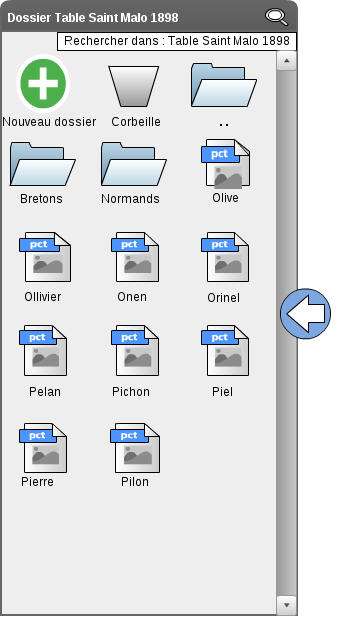
\includegraphics[width=4cm,height=9cm]{interface_mesdocuments.png}
\caption{Interface de gestion des documents}
\label{fig:interface_mesdocuments}
\end{figure}

\begin{table}[H]
  \centering
   \small
	\begin{tabular}{|c|p{12cm}|}
   		\hline
   			\rowcolor{lightgray}\multicolumn{2}{|c|}{\textbf{SD04 - Créer un dossier}} \\
   		\hline
   			\multicolumn{2}{|l|}{Condition de d\'eclenchement} \\
   		\hline
   			-1 & Un utilisateur appuie sur "Nouveau dossier". \\
   		\hline
   			\multicolumn{2}{|l|}{D\'eclenchement de l'op\'eration} \\
   		\hline
   			-1 & L'utilisateur choisit un nom et valide. \\
   		\hline
   			\multicolumn{2}{|l|}{Entrants de l'op\'eration} \\
   		\hline
   			-1 & Dossier parent.\\
        		-2 & Nom\\
   		\hline
   			\multicolumn{2}{|l|}{Traitement de l'op\'eration} \\
  		\hline
   			-1 & Ajout d'une entr\'ee dans la base de donn\'ees. \\
			-2 & Création du nouveau dossier. \\
   		\hline
   			\multicolumn{2}{|l|}{Sortants de l'op\'eration} \\
   		\hline
   			-1 & Le dossier créé. \\
   		\hline
	\end{tabular}
  \caption{SD04 - Créer un dossier}
  \normalsize
  \label{tab:creer_document}
\end{table}

\subsubsection{Fonction SD05 - Renommer un document}
L'utilisateur pourra renommer ses documents à sa guise (sauf "..", "Mes annotations" et "Corbeille"). Cependant, aucun doublon ne sera toléré.

Utilisation : 

\begin{table}[H]
  \centering
   \small
	\begin{tabular}{|c|p{12cm}|}
   		\hline
   			\rowcolor{lightgray}\multicolumn{2}{|c|}{\textbf{SD05 - Renommer un document}} \\
   		\hline
   			\multicolumn{2}{|l|}{Condition de d\'eclenchement} \\
   		\hline
   			-1 & Un utilisateur veut renommer un document.\\
   		\hline
   			\multicolumn{2}{|l|}{D\'eclenchement de l'op\'eration} \\
   		\hline
   			-1 & L'utilisateur  \\
   		\hline
   			\multicolumn{2}{|l|}{Entrants de l'op\'eration} \\
   		\hline
   			-1 & Document (dossier, table ou RMM)\\
        		-2 & Chaîne représentant le nouveau nom\\
   		\hline
   			\multicolumn{2}{|l|}{Traitement de l'op\'eration} \\
  		\hline
   			-1 & Vérification de l'unicité du nom. \\
			-2 & Si valide, remplacement du nom dans la base. \\
			-3 & Si échec, envoi d'un message d'erreur. \\
   		\hline
   			\multicolumn{2}{|l|}{Sortants de l'op\'eration} \\
   		\hline
   			-1 & Si valide, le dossier renommé. \\
			-2 & Si échec, une boîte de dialogue contenant le message d'erreur. \\
   		\hline
	\end{tabular}
  \caption{SD05 - Renommer un document}
  \normalsize
  \label{tab:renommer_document}
\end{table}

\subsubsection{Fonction SD06 - Déplacer un document dans un dossier}
L'utilisateur pourra déplacer s'il le souhaite un document (dossier, table ou RMM) dans un dossier.

Utilisation : l'utilisateur effectue un appui long sur le document choisi, le déplace, en restant appuyé, dans un dossier.

\begin{table}[H]
  \centering
   \small
	\begin{tabular}{|c|p{12cm}|}
   		\hline
   			\rowcolor{lightgray}\multicolumn{2}{|c|}{\textbf{SD06 - Déplacer un document}} \\
   		\hline
   			\multicolumn{2}{|l|}{Condition de d\'eclenchement} \\
   		\hline
   			-1 & Un utilisateur déplace un document.\\
   		\hline
   			\multicolumn{2}{|l|}{D\'eclenchement de l'op\'eration} \\
   		\hline
   			-1 & L'utilisateur relâche la pression sur un dossier.\\
   		\hline
   			\multicolumn{2}{|l|}{Entrants de l'op\'eration} \\
   		\hline
   			-1 & Document (dossier, table ou RMM)\\
        		-2 & Dossier\\
   		\hline
   			\multicolumn{2}{|l|}{Traitement de l'op\'eration} \\
  		\hline
   			-1 & Vérification de l'unicité du nom. \\
			-2 & Si valide, déplace le document dans le dossier. \\
			-3 & Si échec, envoi d'un message d'erreur. \\
   		\hline
   			\multicolumn{2}{|l|}{Sortants de l'op\'eration} \\
   		\hline
   			-1 & Si valide, le dossier déplacé. \\
			-2 & Si échec, une boîte de dialogue contenant le message d'erreur. \\
   		\hline
	\end{tabular}
  \caption{SD06 - Déplacer un document}
  \normalsize
  \label{tab:deplacer_document}
\end{table}

\subsubsection{Fonction SD07 - Supprimer un document}
La suppression fonctionne comme un déplacement, seulement, le document doit être déplacer dans la Corbeille, une boîte de confirmation est envoyée à l'utilisateur.
Si l'utilisateur supprime un dossier, tous les documents présents sont supprimés.
Il est impossible de supprimer le dossier "..", "Mes annotations" et "Corbeille".

Utilisation : l'utilisateur effectue un appui long sur le document choisi, le déplace, en restant appuyé, vers la Corbeille.

\begin{table}[H]
  \centering
   \small
	\begin{tabular}{|c|p{12cm}|}
   		\hline
   			\rowcolor{lightgray}\multicolumn{2}{|c|}{\textbf{SD07 - Supprimer un document}} \\
   		\hline
   			\multicolumn{2}{|l|}{Condition de d\'eclenchement} \\
   		\hline
   			-1 & Un utilisateur déplace un document vers la Corbeille.\\
   		\hline
   			\multicolumn{2}{|l|}{D\'eclenchement de l'op\'eration} \\
   		\hline
   			-1 & L'utilisateur confirme sa suppression.\\
   		\hline
   			\multicolumn{2}{|l|}{Entrants de l'op\'eration} \\
   		\hline
   			-1 & Document (dossier, table ou RMM)\\
        		-2 & Corbeille\\
   		\hline
   			\multicolumn{2}{|l|}{Traitement de l'op\'eration} \\
  		\hline
   			-1 & Si dossier, efface tous les sous documents. \\
			-2 & Si document, efface le document. \\
			-3 & Envoi d'un message d'information. \\		
		\hline
   			\multicolumn{2}{|l|}{Sortants de l'op\'eration} \\
   		\hline
   			-1 & Message d'information. \\
   		\hline
	\end{tabular}
  \caption{SD07 - Supprimer un document}
  \normalsize
  \label{tab:supprimer_document}
\end{table}

\subsection{Recherche}

Pour un utilisateur qui veut trouver un document en particulier, parcourir tous les documents lui même jusqu'à trouver celui qui l'intéresse est trop fastidieux.
C'est pourquoi nous allons proposer un outil de recherche.
Ce dernier se basera non seulement sur les annotations de l'utilisateur, mais aussi sur celles des autres, afin d'avoir les résultats les plus précis possibles.
Afin d'offrir le maximum de flexibilité, la recherche pourra être effectué sur une large variété de paramètres.

\begin{figure}[H]
\centering
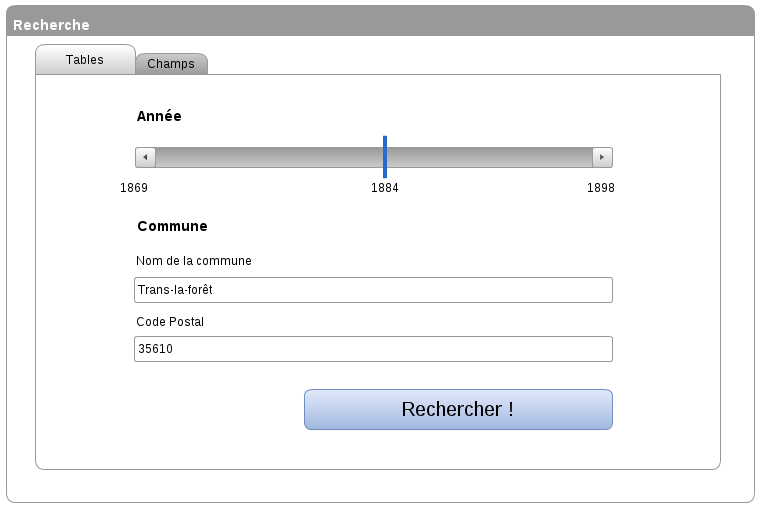
\includegraphics[width=\textwidth]{rechercheTables.png}
\caption{Interface de recherche dans les tables}
\label{fig:rechercheTables}
\end{figure}

\begin{figure}[H]
\centering
\includegraphics[width=\textwidth]{rechercheRMM.png}
\caption{Interface de recherche dans les RMM}
\label{fig:rechercheRMM}
\end{figure}

\subsubsection{Fonction SE01 - Rechercher un nom dans les tables}

L'utilisateur veut trouver le ou les RMM de personnes dont il a le nom. Il peut dans ce cas effectuer une recherche dans les tables grâce à ce nom. Si ce nom a déjà été annoté, l'application propose à l'utilisateur les pages des tables pertinentes. Toutefois ce nom n'est pas toujours repertorié dans les annotations liées aux tables. Si jamais aucune annotation de ce nom existe, l'application propose pour chaque table (chaque année) la page comportant l'annotation du nom la plus proche. Si aucune annotation existe la page ayant le plus de chance d'être la bonne (en suivant l'ordre alphabétique) est proposée.
\\

\begin{table}[H]
  \centering
   \small
	\begin{tabular}{|c|p{12cm}|}
   		\hline
   			\rowcolor{lightgray}\multicolumn{2}{|c|}{\textbf{SE01 - Rechercher un nom dans les tables}} \\
   		\hline
   			\multicolumn{2}{|l|}{Condition de d\'eclenchement} \\
   		\hline
   			-1 & Un utilisateur veut trouver un patronyme dans les tables. \\
   		\hline
   			\multicolumn{2}{|l|}{D\'eclenchement de l'op\'eration} \\
   		\hline
   			-1 & L'utilisateur clique sur le bouton correspondant. \\
   		\hline
   			\multicolumn{2}{|l|}{Entrants de l'op\'eration} \\
   		\hline
   			-1 & Nom \\
   		\hline
   			\multicolumn{2}{|l|}{Traitement de l'op\'eration} \\
  		\hline
  			-1 & Vérification de la validité des champs renseignés. \\
   			-2 & Recherche dans la base de données en fonction des champs renseignés. \\
        	-3 & Affichage des pages qui correspondent à la recherche. \\
   		\hline
   			\multicolumn{2}{|l|}{Sortants de l'op\'eration} \\
   		\hline
   			-1 & Les pages qui correspondent à la recherche. \\
   		\hline
	\end{tabular}
  \caption{SE01 - Rechercher un nom dans les tables}
  \normalsize
  \label{tab:SE01}
\end{table}

\subsubsection{Fonction SE02 - Rechercher des RMM grâce aux annotations générales}

L'utilisateur veut trouver un ou des RMM, non pas en les parcourant un par un mais en utilisant les informations déjà annotées.
\\

\begin{table}[H]
  \centering
   \small
	\begin{tabular}{|c|p{12cm}|}
   		\hline
   			\rowcolor{lightgray}\multicolumn{2}{|c|}{\textbf{SE02 - Rechercher des RMM grâce aux annotations générales}} \\
   		\hline
   			\multicolumn{2}{|l|}{Condition de d\'eclenchement} \\
   		\hline
   			-1 & Un utilisateur veut trouver un RMM en puisant dans la base de données des annotations. \\
   		\hline
   			\multicolumn{2}{|l|}{D\'eclenchement de l'op\'eration} \\
   		\hline
   			-1 & L'utilisateur clique sur le bouton correspondant. \\
   		\hline
   			\multicolumn{2}{|l|}{Entrants de l'op\'eration} \\
   		\hline
   			-1 & Nom et prénom \\
        	-2 & Date de naissance ou classe \\ 
        	-3 & Lieu de recrutement \\
   		\hline
   			\multicolumn{2}{|l|}{Traitement de l'op\'eration} \\
  		\hline
  			-1 & Vérification de la validité des champs renseignés. \\
   			-2 & Recherche dans la base de données en fonction des champs renseignés. \\
        	-3 & Affichage des RMM qui correspondent à la recherche. \\
   		\hline
   			\multicolumn{2}{|l|}{Sortants de l'op\'eration} \\
   		\hline
   			-1 & Les RMM préalablement annotés qui correspondent à la recherche. \\
   		\hline
	\end{tabular}
  \caption{SE02 - Rechercher des RMM grâce aux annotations générales}
  \normalsize
  \label{tab:SE02}
\end{table}

\subsubsection{Fonction SE03 - Rechercher des RMM grâce aux annotations personnelles}

Comme pour la fonction précedente, l'utilisateur veut trouver un ou des RMM en puisant dans la base de données des annotations. En revanche, la recherche ne se fera cette fois que sur les annotations de cet utilisateur. 
\\

\begin{table}[H]
  \centering
   \small
	\begin{tabular}{|c|p{12cm}|}
   		\hline
   			\rowcolor{lightgray}\multicolumn{2}{|c|}{\textbf{SE03 - Rechercher des RMM grâce aux annotations personnelles}} \\
   		\hline
   			\multicolumn{2}{|l|}{Condition de d\'eclenchement} \\
   		\hline
   			-1 & Un utilisateur veut trouver un RMM en puisant dans la base de données des informations qu'il a annoté. \\
   		\hline
   			\multicolumn{2}{|l|}{D\'eclenchement de l'op\'eration} \\
   		\hline
   			-1 & L'utilisateur clique sur le bouton correspondant. \\
   		\hline
   			\multicolumn{2}{|l|}{Entrants de l'op\'eration} \\
   		\hline
   			-1 & Nom et prénom \\
        	-2 & Date de naissance ou classe \\ 
        	-3 & Lieu de recrutement \\ 
   		\hline
   			\multicolumn{2}{|l|}{Traitement de l'op\'eration} \\
  		\hline
  			-1 & Vérification de la validité des champs renseignés. \\
   			-2 & Recherche dans la base de données en fonction des champs renseignés. \\
        	-3 & Affichage des RMM qui correspondent à la recherche. \\
   		\hline
   			\multicolumn{2}{|l|}{Sortants de l'op\'eration} \\
   		\hline
   			-1 & Les RMM préalablement annotés qui correspondent à la recherche. \\
   		\hline
	\end{tabular}
  \caption{SE03 - Rechercher des RMM grâce aux annotations générales}
  \normalsize
  \label{tab:SE03}
\end{table}

\subsubsection{Fonction SE04 - Rechercher un RMM par son numéro matricule.}

L'utilisateur veut trouver un RMM uniquement avec son numéro matricule, sans renseigner son nom, son prénom,\ldots La recherche se fait alors de la même façon que pour les tables : si l'annotation du numéro matricule existe, le RMM est renvoyé. Si l'annotation n'existe pas, l'application estime quel RMM doit être renvoyé en fonction des annotations qui lui sont proches et du nombre d'images.
\\

\begin{table}[H]
  \centering
   \small
	\begin{tabular}{|c|p{12cm}|}
   		\hline
   			\rowcolor{lightgray}\multicolumn{2}{|c|}{\textbf{SE04 - Rechercher un RMM par son numéro matricule}} \\
   		\hline
   			\multicolumn{2}{|l|}{Condition de d\'eclenchement} \\
   		\hline
   			-1 & Un utilisateur veut trouver un RMM grâce à son numéro matricule. \\
   		\hline
   			\multicolumn{2}{|l|}{D\'eclenchement de l'op\'eration} \\
   		\hline
   			-1 & L'utilisateur clique sur le bouton correspondant. \\
   		\hline
   			\multicolumn{2}{|l|}{Entrants de l'op\'eration} \\
   		\hline
   			-1 & Numéro matricule \\
            -2 & Année \\
   		\hline
   			\multicolumn{2}{|l|}{Traitement de l'op\'eration} \\
  		\hline
  			-1 & Vérification de la validité des champs renseignés. \\
   			-2 & Recherche dans la base de données en fonction des champs renseignés. \\
        	-3 & Affichage des pages qui correspondent à la recherche. \\
   		\hline
   			\multicolumn{2}{|l|}{Sortants de l'op\'eration} \\
   		\hline
   			-1 & Les RMM qui correspondent à la recherche. \\
   		\hline
	\end{tabular}
  \caption{SE04 - Rechercher un RMM par son numéro matricule}
  \normalsize
  \label{tab:SE04}
\end{table}

\subsubsection{Fonction SE05 - Rechercher selon un pivot.}

L'utilisateur souhaite obtenir des informations autour de la guerre, par exemple les soldats médaillés ou les blessés à la bataille de la Marne. L'application lui fournit alors, en plus des RMM qui correspondent à sa recherche, des statistiques sur les informations renseignés (nombre de médaillés, \ldots).
\\

\begin{table}[H]
  \centering
   \small
	\begin{tabular}{|c|p{12cm}|}
   		\hline
   			\rowcolor{lightgray}\multicolumn{2}{|c|}{\textbf{SE05 - Rechercher selon un pivot.}} \\
   		\hline
   			\multicolumn{2}{|l|}{Condition de d\'eclenchement} \\
   		\hline
   			-1 & Un utilisateur veut trouver des RMM autour d'un pivot. \\
   		\hline
   			\multicolumn{2}{|l|}{D\'eclenchement de l'op\'eration} \\
   		\hline
   			-1 & L'utilisateur clique sur le bouton correspondant. \\
   		\hline
   			\multicolumn{2}{|l|}{Entrants de l'op\'eration} \\
   		\hline
   			-1 & Médailles \\
            -2 & Régiments \\
            -3 & Blessés \\
            -4 & Batailles \\
   		\hline
   			\multicolumn{2}{|l|}{Traitement de l'op\'eration} \\
  		\hline
  			-1 & Vérification de la validité des champs renseignés. \\
   			-2 & Recherche dans la base de données en fonction des champs renseignés. \\
            -3 & Calcul de statistiques grâce aux résultats de la recherche. \\
        	-4 & Affichage des pages qui correspondent à la recherche. \\
   		\hline
   			\multicolumn{2}{|l|}{Sortants de l'op\'eration} \\
   		\hline
   			-1 & Les RMM qui correspondent à la recherche. \\
            -2 & Les statistiques. \\
   		\hline
	\end{tabular}
  \caption{SE05 - Rechercher selon un pivot.}
  \normalsize
  \label{tab:SE05}
\end{table}

\subsection{Visualisation des documents}

Les images numérisées ne seront pas paramétrées pour un affichage optimal sur l’application, celle-ci devra donc proposer une fonctionnalité proposant la modification de l’affichage d’une image, et non une modification de l’image en elle-même afin de ne pas dégrader l’image originale. En effet, l’image originale peut être d’une taille trop petite ou trop grande, sombre ou mal cadrée, celle-ci dépendant de la qualité l’appareil qui l’a numérisée. Pour faciliter la manipulation de l’affichage de l’image sur l’application, différents outils seront proposés à l’utilisateur : un zoom, une modification du contraste, de la luminosité, d’un effet négatif, de translation en abscisse et ordonnée et de rotation. Pour permettre la conservation des paramètres d’affichage favoris de l’utilisateur, celui-ci pourra les sauvegarder afin d’éviter une manipulation répétitive de ces paramètres. Aussi, un retour à l’état original de l’affichage sera disponible dans le cas où l’utilisateur n’arrive plus à un affichage correct.

D'ailleurs, l'application étant destinée à être tactile, ces fonctionnalités de modification seront accessibles par un raccourci "mouvement", c'est-à-dire que l'utilisateur pourra avec seulement un mouvement de ses doigts exécuter une modification de l'image. Cependant, ces fonctionnalités devront être également accessibles à partir d'une barre d'outils afin de permettre à l'utilisateur de connaître les paramètres qu'il modifient et aussi dans le cas ou l'utilisateur ne sait quel mouvement exécuté.


\subsubsection{Fonction SF01 - Zoom}

Le zoom d'une image permet d'améliorer la lisibilité du document, il permet à l'utilisateur d'agrandir ou de rétricir le document. L'utilisateur pourra paramétrer son zoom selon le pourcentage de la taille de l'image d'origine. Le pourcentage autorisera une modification de 20\% jusqu'à 300\% de la taille de l'image d'origine.
\todo{Question : Faut-il déjà limiter les paramètres ou bien est-ce destiné à la conception ?}

Raccourci mouvement : L'utilisateur colle ses doigts sur une zone de l'image, et les écarte pour agrandir la zone, mouvement inverse pour un rétrécissement.
\todo{Question : Doit-on aussi préciser les mouvements pour le tactile ?}
\todo{Question : Pour le plan du coup il faut peut être dire avant que l'application sera tactile, donc Architecture Générale à mettre avant ? }

\begin{table}[H]
  \centering
   \small
	\begin{tabular}{|c|p{12cm}|}
   		\hline
   			\rowcolor{lightgray}\multicolumn{2}{|c|}{\textbf{SF01 - Fonction Zoom}} \\
   		\hline
   			\multicolumn{2}{|l|}{Condition de d\'eclenchement} \\
   		\hline
   			-1 & Un utilisateur veut zoomer ou dezoomer une image qu'il visionne. \\
   		\hline
   			\multicolumn{2}{|l|}{D\'eclenchement de l'op\'eration} \\
   		\hline
   			-1 & L'utilisateur valide son zoom après l'avoir configuré. \\
   		\hline
   			\multicolumn{2}{|l|}{Entrants de l'op\'eration} \\
   		\hline
   			-1 & Une image \\
        	-2 & Un zoom exprimé en pourcentage de la taille de l'image d'origine \\ 	
        \hline
   			\multicolumn{2}{|l|}{Traitement de l'op\'eration} \\
  		\hline
   			-1 & L'affichage de l'image est modifié (agrandi ou rétréci), selon le pourcentage de la taille de l'image d'origine. \\
   		\hline
   			\multicolumn{2}{|l|}{Sortants de l'op\'eration} \\
   		\hline
   			-1 & L'affichage de l'image modifié \\
   		\hline
	\end{tabular}
  \caption{SF01 - Fonction Zoom}
  \normalsize
  \label{tab:visu_img_zoom}
\end{table}


\subsubsection{Fonction SF02 - Translation}

La translation en abscisse et ordonnée d'une image permet de déplacer l'image par rapport à un certain repère et obtenir ainsi le centrage à l'écran d'une zone partielle ou entière du document. Cette fonctionnalité est destinée à recadrer correctement une image dans le but d'afficher une zone qui intéresserait l'utilisateur.

Raccourci mouvement : L'utilisateur pointe l'image avec un doigt en marquant une pause (pour un effet long), puis est invité à déplacer l'image en déplaçant son doigt.

\begin{table}[H]
  \centering
   \small
	\begin{tabular}{|c|p{12cm}|}
   		\hline
   			\rowcolor{lightgray}\multicolumn{2}{|c|}{\textbf{SF02 - Fonction Translation}} \\
   		\hline
   			\multicolumn{2}{|l|}{Condition de d\'eclenchement} \\
   		\hline
   			-1 & Un utilisateur veut déplacer une image. \\
   		\hline
   			\multicolumn{2}{|l|}{D\'eclenchement de l'op\'eration} \\
   		\hline
   			-1 & L'utilisateur sélectionne l'image et la translate en x et en y par rapport à un repère. \\
   		\hline
   			\multicolumn{2}{|l|}{Entrants de l'op\'eration} \\
   		\hline
        	-1 & Une image \\
   			-2 & Un repère \\
        	-3 & Une translation en x et en y \\ 	
        \hline
   			\multicolumn{2}{|l|}{Traitement de l'op\'eration} \\
  		\hline
   			-1 & L'image est déplacée par rapport au repère et aux translations \\
   		\hline
   			\multicolumn{2}{|l|}{Sortants de l'op\'eration} \\
   		\hline
   			-1 & L'image déplacée \\
   		\hline
	\end{tabular}
  \caption{SF02 - Fonction Translation}
  \normalsize
  \label{tab:visu_img_translation}
\end{table}

\subsubsection{Fonction SF03 - Rotation}

La rotation d'une image permet de faire pivoter l'image dans l'objectif de consulter un objet comme une phrase ou un mot qui serait écrit de travers.

Raccourci mouvement : L'utilisateur positionne deux doigt sur l'image et effectue un mouvement circulaire dans un sens horaire ou anti-horaire.

\begin{table}[H]
  \centering
   \small
	\begin{tabular}{|c|p{12cm}|}
   		\hline
   			\rowcolor{lightgray}\multicolumn{2}{|c|}{\textbf{SF03 - Fonction Rotation}} \\
   		\hline
   			\multicolumn{2}{|l|}{Condition de d\'eclenchement} \\
   		\hline
   			-1 & Un utilisateur veut pivoter une image. \\
   		\hline
   			\multicolumn{2}{|l|}{D\'eclenchement de l'op\'eration} \\
   		\hline
   			-1 & L'utilisateur paramètre son angle de rotation et confirme sa rotation. \\
   		\hline
   			\multicolumn{2}{|l|}{Entrants de l'op\'eration} \\
   		\hline
        	-1 & Une image \\
   			-2 & Un angle de rotation \\ 	
        \hline
   			\multicolumn{2}{|l|}{Traitement de l'op\'eration} \\
  		\hline
   			-1 & L'image est pivotée selon l'angle de rotation \\
   		\hline
   			\multicolumn{2}{|l|}{Sortants de l'op\'eration} \\
   		\hline
   			-1 & L'image pivotée \\
   		\hline
	\end{tabular}
  \caption{SF03 - Fonction Rotation}
  \normalsize
  \label{tab:visu_img_rotation}
\end{table}


\subsubsection{Fonction SF04 - Contraste}

Contraster une image permet de renforcer la différenciation entre les couleurs foncés et les couleurs clairs dans le but d'améliorer la lisibilité de l'image.

Raccourci mouvement : aucun.

\begin{table}[H]
  \centering
   \small
	\begin{tabular}{|c|p{12cm}|}
   		\hline
   			\rowcolor{lightgray}\multicolumn{2}{|c|}{\textbf{SF04 - Fonction Contraste}} \\
   		\hline
   			\multicolumn{2}{|l|}{Condition de d\'eclenchement} \\
   		\hline
   			-1 & Un utilisateur veut contraster une image. \\
   		\hline
   			\multicolumn{2}{|l|}{D\'eclenchement de l'op\'eration} \\
   		\hline
   			-1 & L'utilisateur paramètre son contraste et le confirme. \\
   		\hline
   			\multicolumn{2}{|l|}{Entrants de l'op\'eration} \\
   		\hline
        	-1 & Une image \\
   			-2 & Un contraste \\ 	
        \hline
   			\multicolumn{2}{|l|}{Traitement de l'op\'eration} \\
  		\hline
   			-1 & L'image est contrastée selon le contraste donné en paramètre \\
   		\hline
   			\multicolumn{2}{|l|}{Sortants de l'op\'eration} \\
   		\hline
   			-1 & L'image contrastée \\
   		\hline
	\end{tabular}
  \caption{SF04 - Fonction Contraste}
  \normalsize
  \label{tab:visu_img_contraste}
\end{table}



\subsubsection{Fonction SF05 - Luminosité}


Augmenter ou diminuer la luminosité d'une image améliorer la netteté et donc la lisibilité de l'image.

Raccourci mouvement : aucun.

\begin{table}[H]
  \centering
   \small
	\begin{tabular}{|c|p{12cm}|}
   		\hline
   			\rowcolor{lightgray}\multicolumn{2}{|c|}{\textbf{SF05 - Fonction Luminosité}} \\
   		\hline
   			\multicolumn{2}{|l|}{Condition de d\'eclenchement} \\
   		\hline
   			-1 & Un utilisateur veut augmenter ou diminuer la luminosité d'une image. \\
   		\hline
   			\multicolumn{2}{|l|}{D\'eclenchement de l'op\'eration} \\
   		\hline
   			-1 & L'utilisateur sa luminosité et confirme. \\
   		\hline
   			\multicolumn{2}{|l|}{Entrants de l'op\'eration} \\
   		\hline
        	-1 & Une image \\
   			-2 & Une luminosité \\ 	
        \hline
   			\multicolumn{2}{|l|}{Traitement de l'op\'eration} \\
  		\hline
   			-1 & L'image est modifiée selon la luminosité donnée en paramètre \\
   		\hline
   			\multicolumn{2}{|l|}{Sortants de l'op\'eration} \\
   		\hline
   			-1 & L'image modifiée \\
   		\hline
	\end{tabular}
  \caption{SF05 - Fonction Luminosité}
  \normalsize
  \label{tab:visu_img_luminosite}
\end{table}

\subsubsection{Fonction SF06 - Défaire / Refaire}

Lorsque l'utilisateur hésite quant à sa modification de l'image, il paraît nécessaire que celui-ci puisse annuler, défaire son changement pour revenir à l'état précédent de l'image. Aussi, il pourra refaire son changement s'il le souhaite, ce sont des raccourcis efficaces qui évite plusieurs manipulations par l'utilisateur.

Raccourci mouvement : aucun.

\begin{table}[H]
  \centering
   \small
	\begin{tabular}{|c|p{12cm}|}
   		\hline
   			\rowcolor{lightgray}\multicolumn{2}{|c|}{\textbf{SF06 - Fonction Défaire / Refaire}} \\
   		\hline
   			\multicolumn{2}{|l|}{Condition de d\'eclenchement} \\
   		\hline
   			-1 & Un utilisateur veut annuler ou refaire sa manipulation de l'image. \\
   		\hline
   			\multicolumn{2}{|l|}{D\'eclenchement de l'op\'eration} \\
   		\hline
   			-1 & L'utilisateur confirme. \\
   		\hline
   			\multicolumn{2}{|l|}{Entrants de l'op\'eration} \\
   		\hline
        	-1 & Une image \\
   			-2 & Une action \\ 	
        \hline
   			\multicolumn{2}{|l|}{Traitement de l'op\'eration} \\
  		\hline
   			-1 & L'image défait ou refait l'action \\
   		\hline
   			\multicolumn{2}{|l|}{Sortants de l'op\'eration} \\
   		\hline
   			-1 & L'image modifiée \\
   		\hline
	\end{tabular}
  \caption{SF06 - Fonction Défaire / Refaire}
  \normalsize
  \label{tab:visu_img_undo_redo}
\end{table}



\subsubsection{Fonction SF07 - Sauvegarder les paramètres}

L'utilisateur pourra sauvegarder ses paramètres préférentiels dans un raccourci, afin d'éviter de répéter différentes manipulations lorqu'il consulte plusieurs images. Celui-ci pourra donc refaire toutes ses manipulations en une seule actio, augmentant l'efficacité d'utilisation de l'application.

Raccourci mouvement : aucun.

\begin{table}[H]
  \centering
   \small
	\begin{tabular}{|c|p{12cm}|}
   		\hline
   			\rowcolor{lightgray}\multicolumn{2}{|c|}{\textbf{SF07 - Fonction Sauvegarder les paramètres}} \\
   		\hline
   			\multicolumn{2}{|l|}{Condition de d\'eclenchement} \\
   		\hline
   			-1 & Un utilisateur souhaite conserver les paramètres actuels. \\
   		\hline
   			\multicolumn{2}{|l|}{D\'eclenchement de l'op\'eration} \\
   		\hline
   			-1 & L'utilisateur confirme. \\
   		\hline
   			\multicolumn{2}{|l|}{Entrants de l'op\'eration} \\
   		\hline
        	-1 & Une liste d'action \\ 	
        \hline
   			\multicolumn{2}{|l|}{Traitement de l'op\'eration} \\
  		\hline
   			-1 & L'application conserve en local cette liste d'action \\
   		\hline
   			\multicolumn{2}{|l|}{Sortants de l'op\'eration} \\
   		\hline
   			-1 & Un raccourci permettant d'exécuter les actions stockées dans la liste \\
   		\hline
	\end{tabular}
  \caption{SF07 - Fonction Sauvegarder les paramètres}
  \normalsize
  \label{tab:visu_img_save_parameters}
\end{table}

\subsection{Administration}

Comme nous avons pu le voir précédemment, les utilisateurs authentifiés sont divisés en 3 catégories : les utilisateurs basiques, les modérateurs et les administrateurs. Les modérateurs sont présents dans l'objectif de supprimer un utilisateur basique ou de masquer les annotations de certains utilisateurs. Quant à l'administrateur, il a les droits du modérateur mais ils ont aussi la possibilité de modifier le statut des utilisateurs et de supprimer tout type d'utilisateur, y-compris les modérateurs et administrateurs. Afin de permettre la gestion des utilisateurs, il existera une interface d'administration.

\subsubsection{Fonction SG01 - Supprimer un ou des utilisateurs basiques}

Les modérateurs peuvent supprimer un utilisateur basique de la base de données. Ceci se fait au travers de la page de gestion des utilisateurs. Le modérateur sélectionne les utilisateurs qu'il souhaite supprimer puis il les supprime.

\begin{table}[H]
  \centering
   \small
	\begin{tabular}{|c|p{12cm}|}
   		\hline
   			\rowcolor{lightgray}\multicolumn{2}{|c|}{\textbf{Fonction SG01 - Supprimer un ou des utilisateurs}} \\
   		\hline
   			\multicolumn{2}{|l|}{Condition de déclenchement} \\
   		\hline
   			-1 & L'utilisateur a le status de modérateur.\\
        			-2 & L'utilisateur est sur la page de gestion des utilisateurs et souhaite supprimer une liste d'utilisateurs basiques.\\
        
   		\hline
   			\multicolumn{2}{|l|}{Déclenchement de l'opération} \\
   		\hline
   			-1 & L'utilisateur modérateur sélectionne un ou des utilisateurs basiques et les supprime.\\
   		\hline
   			\multicolumn{2}{|l|}{Entrants de l'opération} \\
   		\hline
   			-1 & Une liste d'utilisateurs basiques\\
   		\hline
   			\multicolumn{2}{|l|}{Traitement de l'opération} \\
  		\hline
   			-1 & Suppression des utilisateurs de la base de donnée.\\
   		\hline
   			\multicolumn{2}{|l|}{Sortants de l'opération} \\
   		\hline
   			-1 & Renvoi vers la page de gestion des utilisateurs.\\
        			-2 & Renvoi d'une erreur si échec.\\ 
   		\hline
	\end{tabular}
  \caption{Fonction SG01 - Supprimer un ou des utilisateurs basiques}
  \normalsize
  \label{tab: supprimmer_utilisateur_basique}
\end{table}


\subsubsection{Fonction SG02 - Desactiver les annotations d'un ou plusieurs utilisateur}

Les annotations de certains utilisateurs peuvent induire en erreur d'autres utilisateurs. Pour éviter cela, les modérateurs doivent avoir la possibilité de désactiver les annotations de certains utilisateurs sans pour autant les banir. Cette désactivation empêche la visibilité des annoations par les autres utilisateurs. Un administrateur a la possibilité d'effectuer cette action via la page de gestion des utilisateurs. 

\begin{table}[H]
  \centering
   \small
	\begin{tabular}{|c|p{12cm}|}
   		\hline
   			\rowcolor{lightgray}\multicolumn{2}{|c|}{\textbf{Fonction SG02 - Desactiver les annotations d'un ou plusieurs utilisateur}} \\
   		\hline
   			\multicolumn{2}{|l|}{Condition de déclenchement} \\
   		\hline
   			-1 & L'utilisateur a le status de modérateur.\\
        	-2 & L'utilisateur est sur la page de gestion des utilisateurs et souhaite désactiver la visibilité des annocations d'une liste d'utilisateurs.\\
   		\hline
   			\multicolumn{2}{|l|}{Déclenchement de l'opération} \\
   		\hline
   			-1 & L'utilisateur modérateur sélectionne un ou des utilisateurs de la liste et désactive la visibilité de leurs annotations.\\
   		\hline
   			\multicolumn{2}{|l|}{Entrants de l'opération} \\
   		\hline
   			-1 & Une liste d'utilisateurs\\
   		\hline
   			\multicolumn{2}{|l|}{Traitement de l'opération} \\
  		\hline
   			-1 & Un champ "visiblité" de la base de donnée est mis à faux pour les utilisateurs en question.\\
   		\hline
   			\multicolumn{2}{|l|}{Sortants de l'opération} \\
   		\hline
   			-1 & Renvoi vers la page de gestion des utilisateurs.\\
        	-2 & Renvoi d'une erreur si échec.\\
   		\hline
	\end{tabular}
  \caption{Fonction SG02 - Desactiver les annotations d'un ou plusieurs utilisateur}
  \normalsize
  \label{tab: desactiver_utilisateur}
\end{table}

\subsubsection{Fonction SG03 - Supprimer un ou des utilisateurs ayant le statut de modérateur ou administrateur}

Les administrateurs peuvent, en plus de supprimer un utilisateur basique, supprimer un utilisateur ayant le statut de modérateur ou administrateur. Ceci se fait toujours au travers de la page de gestion des utilisateurs. L'administrateur sélectionne les utilisateurs qu'il souhaite supprimer puis il confirme sa demande.

\begin{table}[H]
  \centering
   \small
	\begin{tabular}{|c|p{12cm}|}
   		\hline
   			\rowcolor{lightgray}\multicolumn{2}{|c|}{\textbf{Fonction SG03 - Supprimer un ou des utilisateurs}} \\
   		\hline
   			\multicolumn{2}{|l|}{Condition de déclenchement} \\
   		\hline
   			-1 & L'utilisateur a le status d'administrateur.\\
        			-2 & L'utilisateur est sur la page de gestion des utilisateurs et souhaite supprimer une liste d'utilisateurs.\\
   		\hline
   			\multicolumn{2}{|l|}{Déclenchement de l'opération} \\
   		\hline
   			-1 & L'utilisateur administrateur sélectionne un ou des utilisateurs basiques et les supprime.\\
   		\hline
   			\multicolumn{2}{|l|}{Entrants de l'opération} \\
   		\hline
   			-1 & Une liste d'utilisateurs\\
   		\hline
   			\multicolumn{2}{|l|}{Traitement de l'opération} \\
  		\hline
   			-1 & Suppression des utilisateurs de la base de donnée.\\
   		\hline
   			\multicolumn{2}{|l|}{Sortants de l'opération} \\
   		\hline
   			-1 & Renvoi vers la page de gestion des utilisateurs.\\
        			-2 & Renvoi d'une erreur si échec.\\ 
   		\hline
	\end{tabular}
  \caption{Fonction SG03 - Supprimer un ou des utilisateurs, quelque soit son statut}
  \normalsize
  \label{tab: supprimmer_utilisateur}
\end{table}

\subsubsection{Fonction SG04 - Changer le rang d'un utilisateur}

Les équipes de modérateurs et d'administrateurs doivent pouvoir évoluer au fil du temps. Pour cela, un administrateur peut changer le rang d'un utilisateur dans l'objectif de le promouvoir modérateur ou administrateur mais il a aussi la possiblité de lui retirer ses droits de modérateur ou d'administrateur si celui-ci les possède.

\begin{table}[H]
  \centering
   \small
	\begin{tabular}{|c|p{12cm}|}
   		\hline
   			\rowcolor{lightgray}\multicolumn{2}{|c|}{\textbf{Fonction SG04 - Changer le rang d'un utilisateur}} \\
   		\hline
   			\multicolumn{2}{|l|}{Condition de déclenchement} \\
   		\hline
   			-1 & L'utilisateur a le status d'administrateur.\\
        	-2 & L'utilisateur est sur la page de gestion des utilisateurs et souhaite changer le rang d'un utilisateur.\\
   		\hline
   			\multicolumn{2}{|l|}{Déclenchement de l'opération} \\
   		\hline
   			-1 & L'utilisateur administrateur sélectionne un utilisateur de la liste et choisi son nouveau rang.\\
   		\hline
   			\multicolumn{2}{|l|}{Entrants de l'opération} \\
   		\hline
   			-1 & Un utilisateur\\
            -2 & Un rang\\
   		\hline
   			\multicolumn{2}{|l|}{Traitement de l'opération} \\
  		\hline
   			-1 & Le nouveau rang écrase l'ancien rang de l'utilisateur dans la base de donnée.\\
   		\hline
   			\multicolumn{2}{|l|}{Sortants de l'opération} \\
   		\hline
   			-1 & Renvoi vers la page de gestion des utilisateurs.\\
        	-2 & Renvoi d'une erreur si échec.\\
   		\hline
	\end{tabular}
  \caption{Fonction SG04 - Changer le rang d'un utilisateur}
  \normalsize
  \label{tab: promouvoir_utilisateur}
\end{table}

\newpage
\section*{Conclusion}

Dans la perspective du centenaire de la guerre 14-18, ce projet a pour objectif de concevoir un outil de navigation, d'annotation et de recherche dans les RMM.

Cette phase de spécifications fonctionnelles nous a permis de formuler précisément les fonctionnalités à développer, ainsi que les interactions qui peuvent exister entre les différentes fonctionnalités. A l'issu de ce rapport, nous avons aussi une idée de l'architecture générale qu'utilisera notre système. A présent, il va être nécessaire de chiffrer le temps de réalisation de ces fonctionnalités dans l'objectif de planifier la conception et le développement de notre système.

\appendix

\section{Vue compl\`ete d'un RMM}
\label{sec:annexe 1}

\begin{figure}[H]
\centering
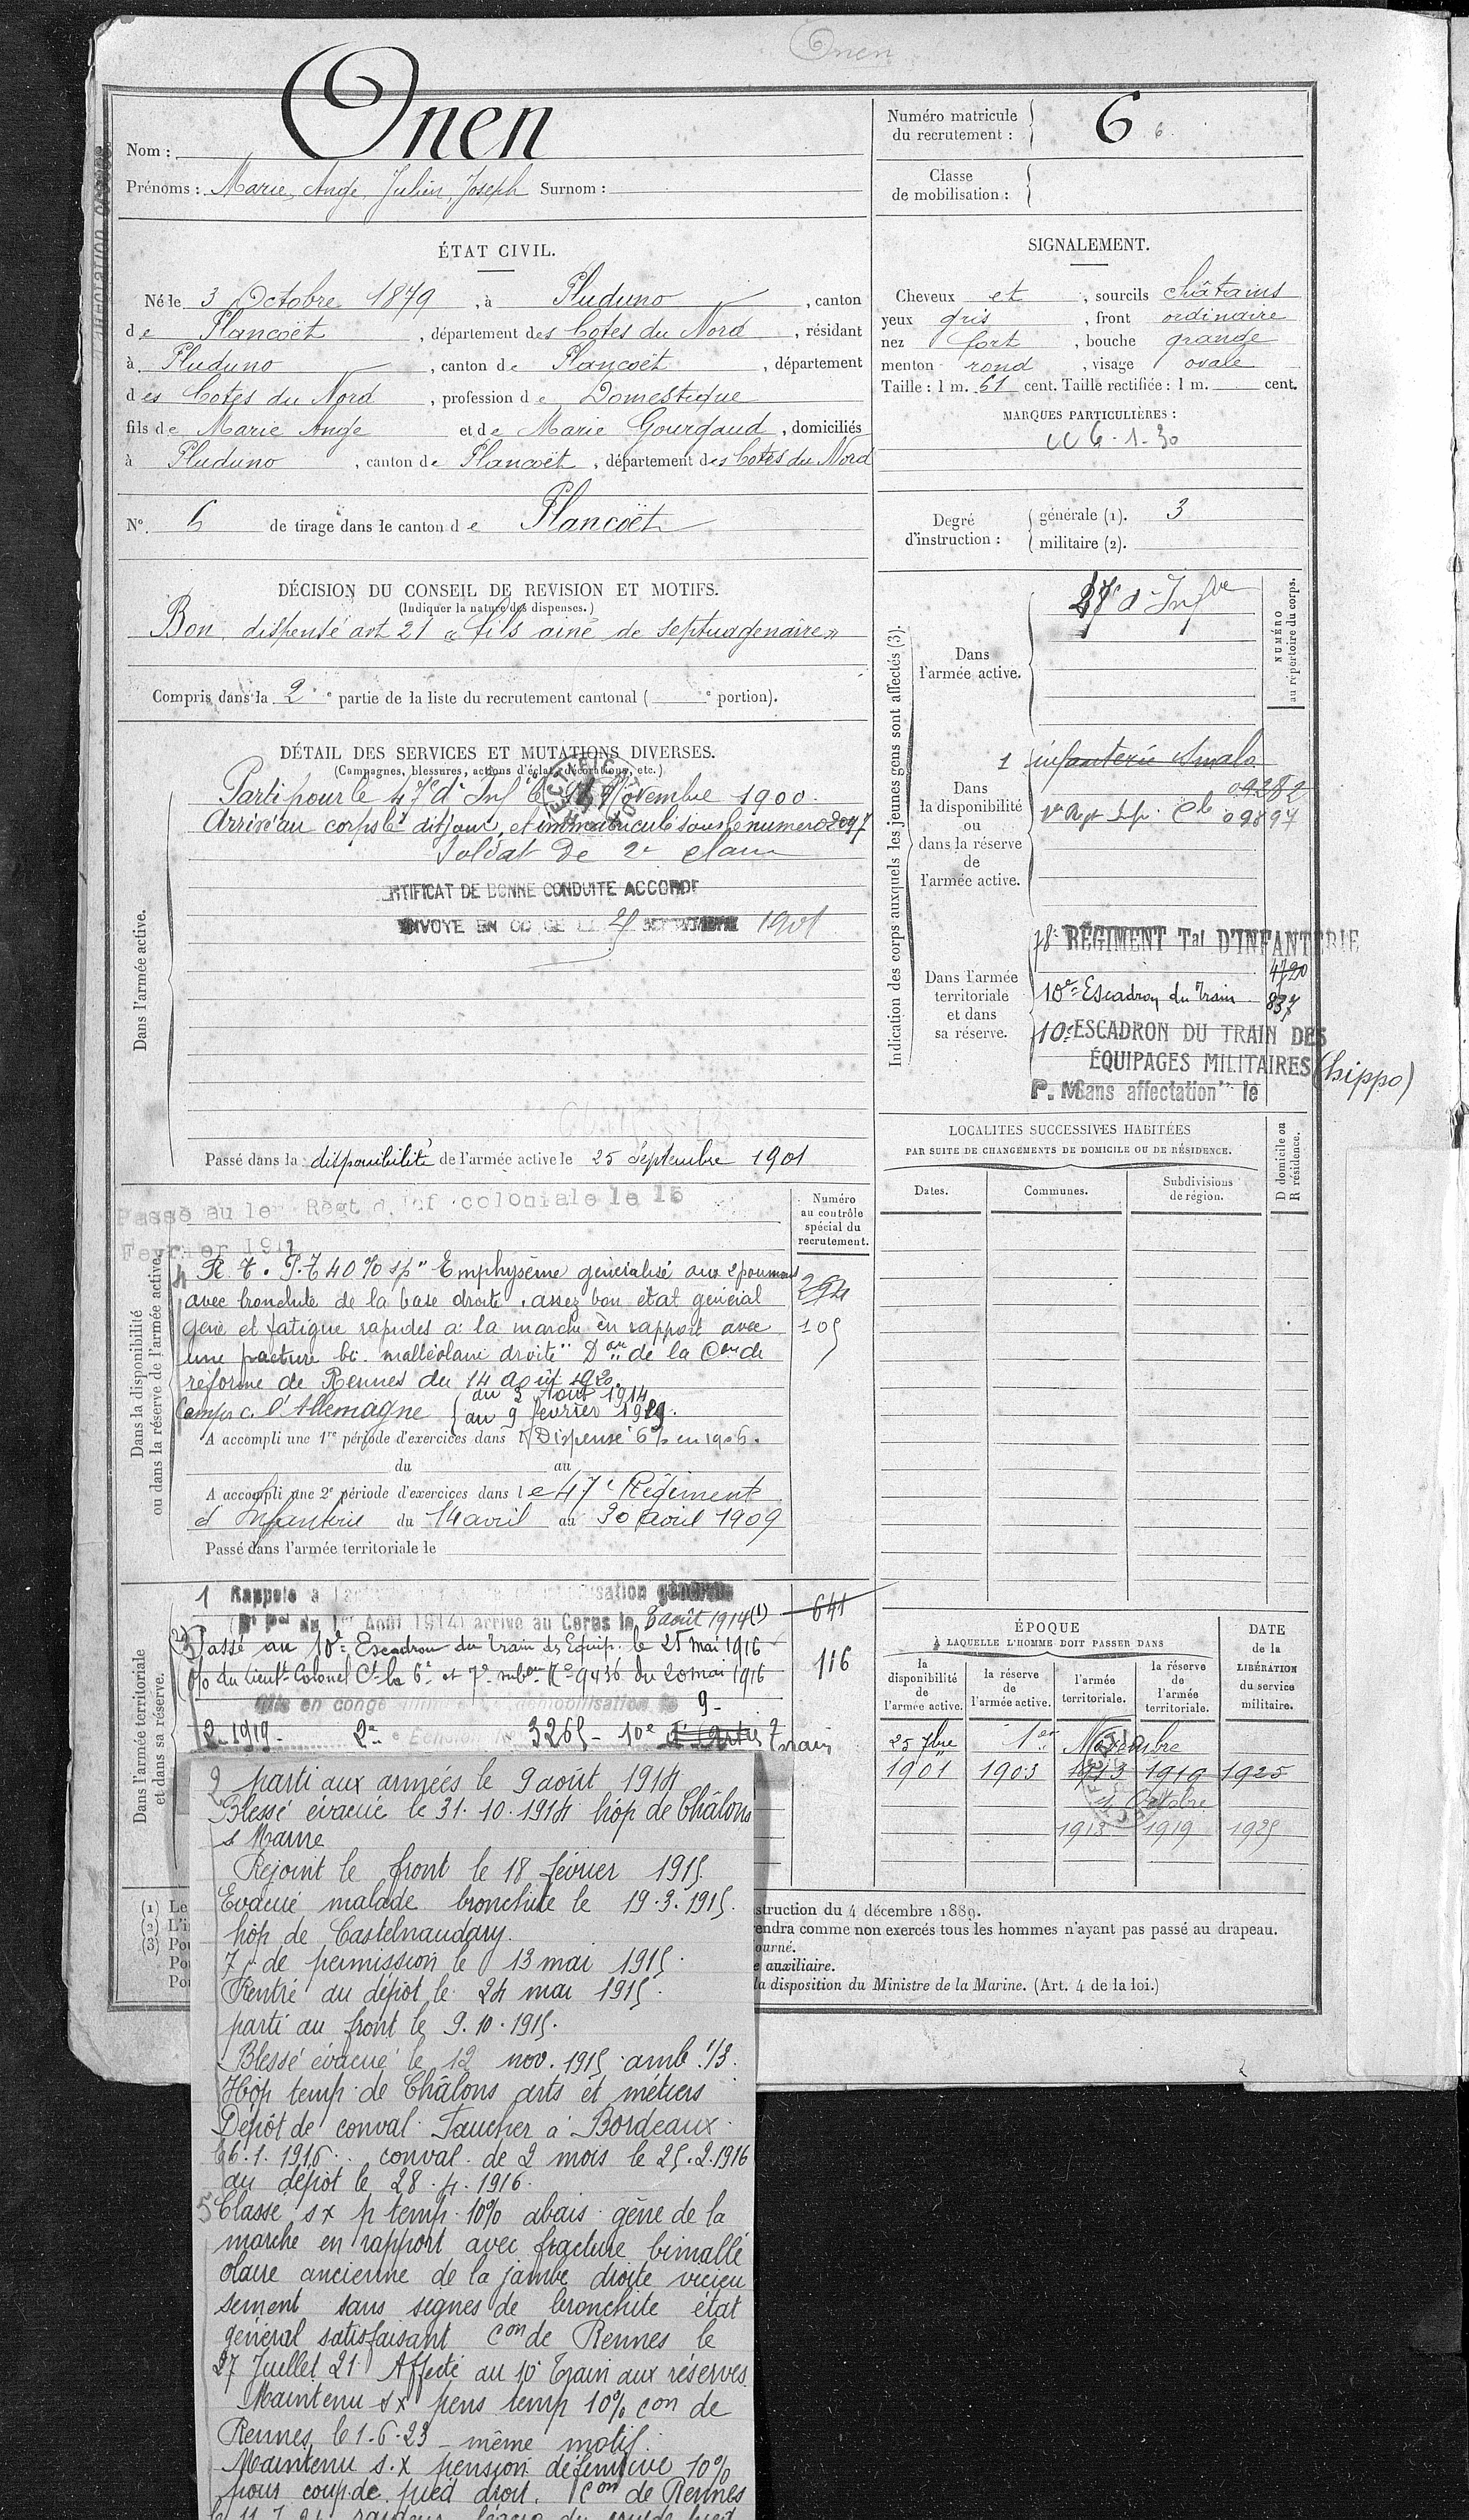
\includegraphics[width=0.95\textwidth]{RMM.JPG}
\end{figure}

\section{Table de RMM - Saint-Malo 1899}
\label{sec:annexe 2}

\begin{figure}[H]
\centering
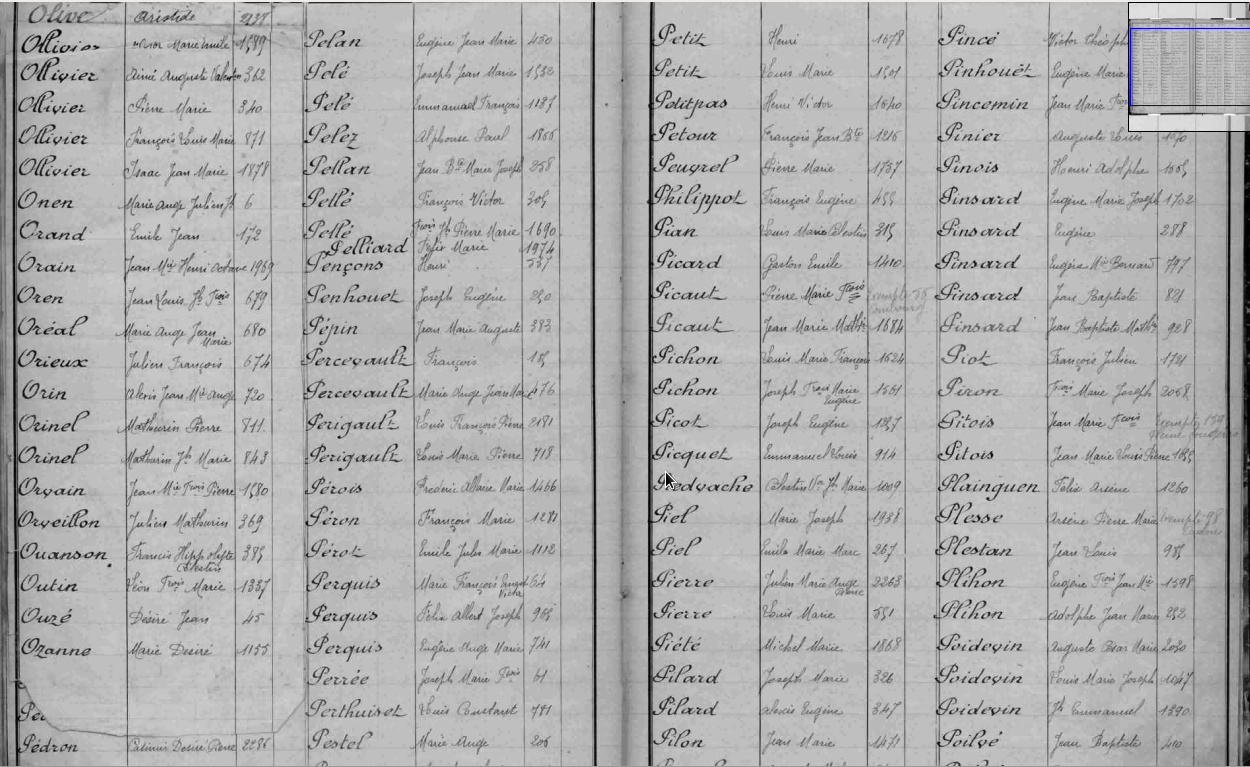
\includegraphics[width=\textwidth]{Table_Onen.png}
\end{figure}
\end{document}
